\documentclass[10pt]{book}
\usepackage{cite}
\usepackage{hyperref}
\usepackage{amsmath}
\usepackage{amsfonts}
\usepackage{graphicx}
\usepackage{enumitem}
\usepackage{multicol}
\usepackage{float}
\usepackage[font=small,labelfont=bf]{caption}
\hypersetup{colorlinks = true}

\author{Alberto Paoluzzi, Francesco Furiani, Giulio Martella}
\title{LARLIB.jl}

\begin{document}

\frontmatter
\maketitle

\section*{Book structure}

This book has two parts: Introduction and Implementation.

The first chapter of the Introduction explain what LAR is
and explores the finalities and goals of LARLIB.jl. The other 
chapters focus on explaining the algorithms behind LAR.

The Implementation part start with a brief overview of the
LARLIB.jl module and the conventions used throughout the module.
The chapters following contain the in-deep
explanation of the code inside each source file of LARLIB.jl;
most of the content is paired with test sets: these are
embedded into the relative chapters. The last chapter
contains the utilities function used everywhere inside LARLIB.jl.

\tableofcontents

\mainmatter

\part{Introduction}
\chapter{LAR}
\label{sec:LAR}

LAR is a general representation scheme for geometric and topological
modeling~\cite{Dicarlo:2014:TNL:2543138.2543294}. 
The domain of the scheme is provided by \textit{cellular complexes}
while its codomain is a set of \textit{sparse matrices}.
The main advantages of the scheme are:
\begin{enumerate}
    \item
    \textit{It is extremely effective to easily represent general non-manifold solids.}
    For example, the memory representation of a $d=3$ cellular complex using LAR 
    consists in only two binary sparse matrices for the topology and a bi-dimensional
    array for the geometry.
    \item
    \textit{Computation and analysis of cellular complexes is
    done only through easy linear algebra operations.} 
    The most common operation is the sparse matrix-vector 
    multiplication.
\end{enumerate}

In LAR we talk about cellular complexes which are made of cells, so we
call $d$-cell the $d$-dimensional cell: 0-cells are vertices,
1-cells are edges, 2-cells are faces, and so on.
Throughout this thesis, these names are completely
interchangeable.

An important concept is represented by the \textit{boundary} and 
\textit{coboundary operators}. They express the relation
between the cells of different dimension but of the same cellular complex.
Even these operators are stored in memory as sparse matrices 
and they can be applied using just a matrix multiplication.

The relation $\partial_d = \delta_{d-1}^\top$ (where $\partial_d$ 
is the $d$-boundary and $\delta_{d-1}$ is the $(d-1)$-coboundary)
is particularly handy. So, for example a 2-boundary expresses 
the relation from the edges to the faces of the same complex and
its transpose is the 1-coboundary that maps faces to edges.

An another concept of LAR used a lot in this thesis is the one of
\textit{skeleton}. A $(d-1)$-skeleton is the set of $(d-1)$-cells of
a $d$-complex. For example, a 2-skeleton of a 3-complex is the set
of all the faces of the complex.

\section{LAR fundamentals}
\label{sec:fundamentals}

\paragraph{LAR model}
A LAR model is a pair \emph{geometry, topology}. The \emph{geometry} is specified by the  position vectors of \emph{vertices} in a Euclidean space $\E^d$ of points with $d$ coordinates. The \emph{topology} is specified by one or more bases of singleton $k$-chains (i.e.~$k$-cells) for $0 \leq k\leq d$. The vertex sharing between cells implicitly provide the attachment maps between cells of various dimensions.
Vertex positions are represented, by rows, by a 2-array of d real coordinates.

\paragraph{Chains as arrays}
Chain-based modeling and computing is based on representation of $p$-cell subsets as \emph{chains}, elements of \emph{linear} spaces $C_p$ ($0\leq p\leq d$) generated by the space decomposition induced by a \emph{cellular complex}, also said \emph{CW- complex}.
Chains can be simply represented as arrays of signed integers, one of simplest and more efficient data structure of most languages, particularly when oriented to scientific computing.
Therefore, basic algebraic operations on chains as vectors (sum and product times a scalar) are implemented over arrays.

\paragraph{Characteristic matrices}
The LAR \emph{representation scheme}~\cite{Requicha:1980:RRS:356827.356833}, i.e.~our mapping between mathematical models of solids and their computer representations, uses linear \emph{chain spaces} $C_p$ as models, and sparse \emph{characteristic matrices} $M_p$  of $p$-cells as symbolic representations, where the $p$-cell $\sigma^k\in\Lambda_p$ is represented as the $k$-th binary row of the  sparse characteristic matrix $M_p: C_0\to C_p$.

\paragraph{Boundary and coboundary matrices}

The boundary matrix $[\partial_p]$ is the matrix of the boundary operator $\partial_p: C_p\to C_{p-1}$ ($1\leq p\leq d$) that for each \emph{chain} $c_p\in C_p$ returns the  boundary $(p-1)$-cycle of its $(d-1)$-faces.  A boundary operator is linear: $\partial_p c + d = \partial_p c + \partial_p d$, for each $c,d\in C_p$. A cycle is a chain without boundary. Hence, t\emph{he} boundary of a boundary is the zero map: $partial_{p-1} \circ partial_p = 0$ ($2\leq p\leq d$).

\paragraph{Incidence matrices}
Incidence operators between chain spaces of different dimension are easy to compute by matrix products of characteristic matrices (see Section~\ref{matrices}), possibly transposed.
Since both characteristic and operator matrices are very sparse, their products are computed with  specialized algorithms for very sparse matrices, whose complexity is roughly linear in the size of the output sparse matrix, i.e., in the number of its stored non-zero elements.
Incidence queries and other types of geometric or topological computations are not performed element-wise, that necessarily require iterative or recursive programming patterns, but only require matrix product times whole chains (sets of cells), so adapting naturally to parallel and/or dataflow computational patterns found in HPC and CNN architectures.

\paragraph{Validity test of a representation}
Data validity is easy to test by checking for satisfaction of basic equations $\partial\partial=\emptyset$ of a chain complex.




\section{Data structures and transformations}
\label{sec:datastructures}



In this section we introduce the basic data objects of the \texttt{LARLIB} module,
i.e., incidence relations, chain bases, and chain transformations. The ground concept of a \emph{chain complex} is a cellular decomposition of a $d$-space into sets of connected $p$-cells ($0\leq p\leq\ d$). 



\subsection{Examples}
\label{sec:examples}

\begin{example}[3D cubical mesh]
\label{ex:boundary1}


A very simple example of 3D cubical mesh is given here. When considered as a solid model,  a \emph{boundary representation} would be normally applied to it. If used as the domain of a simulation, a \emph{decompositive representation} would be usually chosen. Both can be derived by the LAR scheme, given below. A picture of the mesh with numbered $p$-cells in different colors ($0\leq p\leq 3$) is shown in Figure~\ref{fig:intro-1}.

%-------------------------------------------------------------------------------
@d LAR decompositive representation 
@{using LARVIEW

# Simple mesh of two 3-cuboids
V,cells = LARLIB.larCuboids([2,1,1],true)
VV,EV,FV,CV = cells
larmodel = V,(VV,EV,FV,CV)
LARVIEW.viewnumbered(larmodel)
@}
%-------------------------------------------------------------------------------

\begin{figure}[htbp] %  figure placement: here, top, bottom, or page
   \centering
   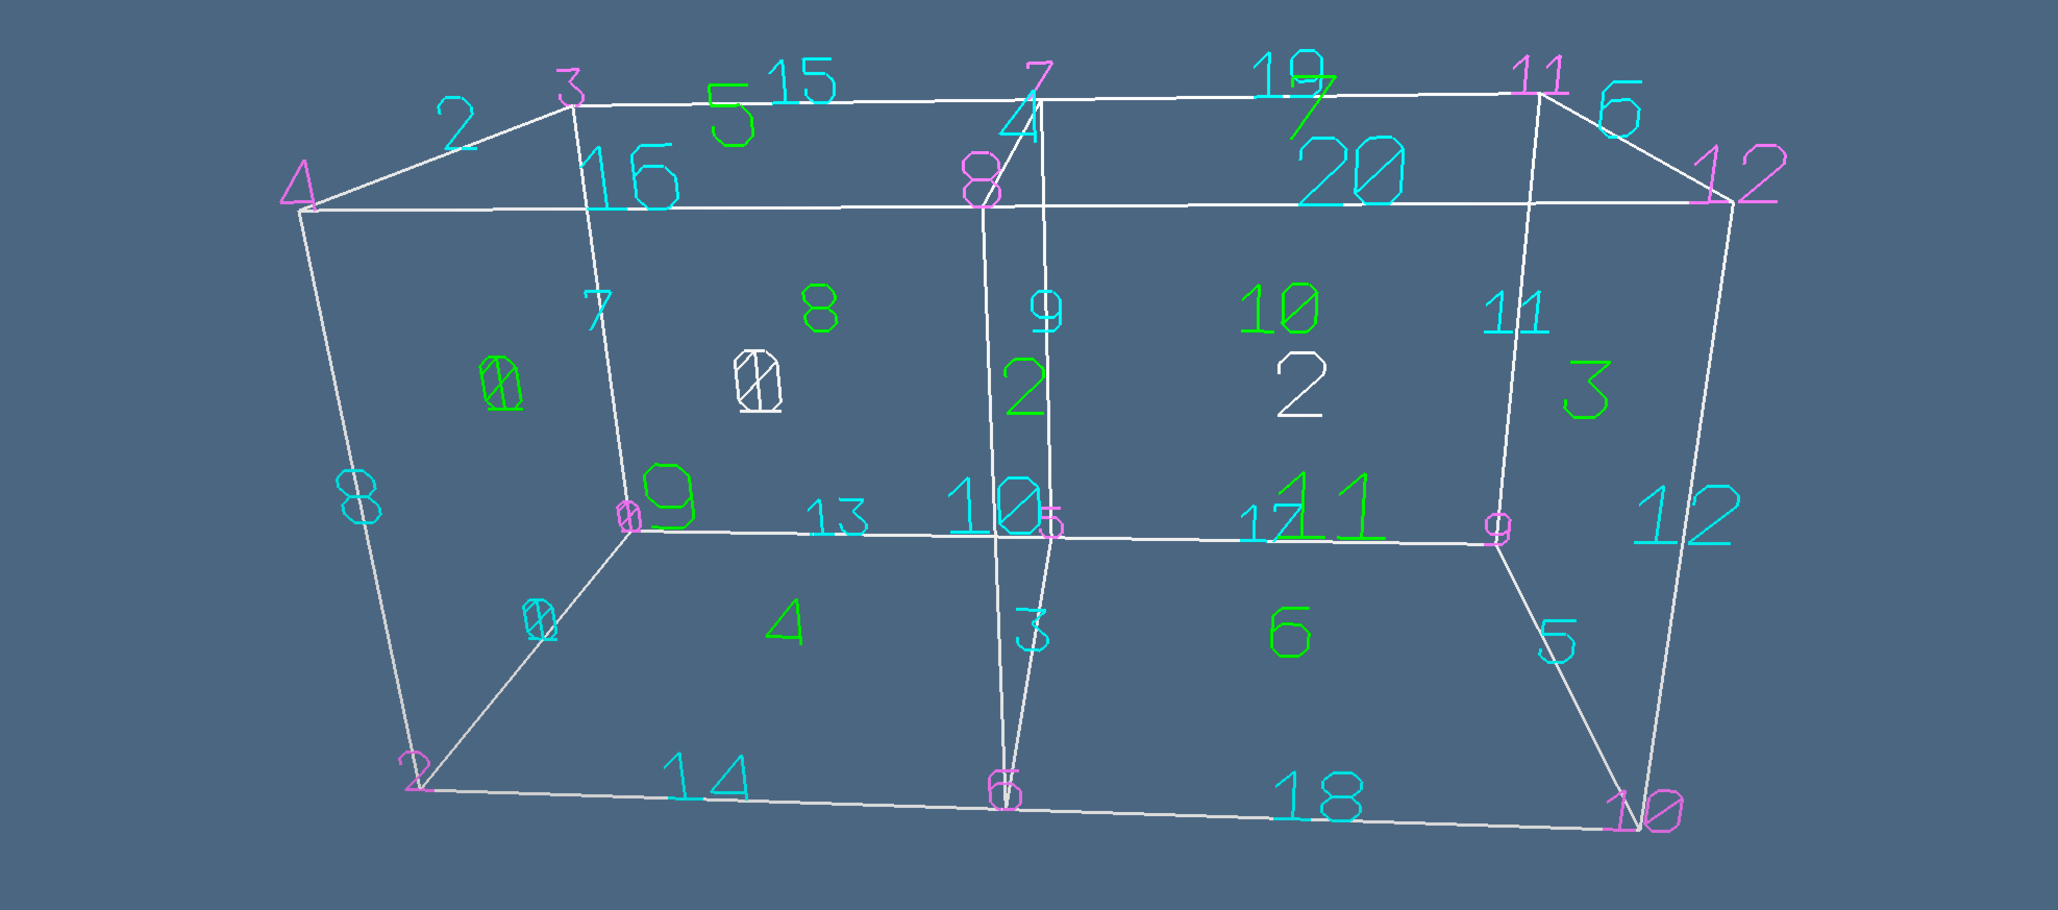
\includegraphics[width=\textwidth]{img/intro-1.pdf} 
   \caption{A cubical 3-mesh with two 3-cells. Notice that $p$-cells of index 1 are also indexed by 0 in the picture, due to (current) incompatibilities by the \texttt{pyplasm} library, used for mesh drawing, and Julia.}
   \label{fig:intro-1}
\end{figure}

The geometric embedding of the grid, given the array $V$ of vertices, and the indexing of $p$-cells as subsets of vertices are given below.

{\small\begin{verbatim}
julia> V
3�12 Array{Int64,2}:
 0  0  0  0  1  1  1  1  2  2  2  2
 0  0  1  1  0  0  1  1  0  0  1  1
 0  1  0  1  0  1  0  1  0  1  0  1
julia> print(VV)
Array{Int64,1}[[1],[2],[3],[4],[5],[6],[7],[8],[9],[10],[11],[12]]
julia> print(EV)
Array{Int64,1}[[1,2],[3,4],[5,6],[7,8],[9,10],[11,12],[1,3],[2,4],[5,7],
[6,8],[9,11],[10,12],[1,5],[2,6],[3,7],[4,8],[5,9],[6,10],[7,11],[8,12]]
julia> print(FV)
Array{Int64,1}[[1,2,3,4],[5,6,7,8],[9,10,11,12],[1,2,5,6],[3,4,7,8],
[5,6,9,10],[7,8,11,12],[1,3,5,7],[2,4,6,8],[5,7,9,11],[6,8,10,12]]
julia> print(CV)
Array{Int64,1}[[1,2,3,4,5,6,7,8],[5,6,7,8,9,10,11,12]]
\end{verbatim}
}
\end{example}

\begin{example}[Input/output of space arrangement algorithm]
\end{example}



\subsection{Data structures}

\label{sec:data} All data structures are either arrays, or sparse arrays, or arrays of arrays. We introduce here some stardard notations, largely used in the following. In particular, we use the symbols \texttt{V}, \texttt{E}, \texttt{F}, \texttt{C}, to denote the arrays of \emph{vertices}, \emph{edges}, \emph{faces}, and \emph{cells},  i.e., to denote the 0-, 1-, 2-, and 3-cells, respectively. 

With some abuse of language, each \emph{$p$-cell} or \emph{elementary $p$-chain} is represented as the \texttt{Array\{Int64,1\}} of the integer indices of its $(p-1)$-faces, either signed or non-signed depending on the consideration of the orientations of the cells.


\paragraph{Incidence relations}

By definition of cellular complex, a $q$-cell $\tau$ and a $r$-cell $\sigma$, with $q\leq r$, either do not intersect or share a common \emph{$p$-face} ($0\leq p\leq q,r$).

Hence in 3D we may consider up to $16=4\times 4$ binary incidence relations between $V,E,F,C$, denoted respectively \texttt{VV}, \texttt{VE}, \texttt{VF}, \texttt{VC}, and
\texttt{EV}, \texttt{EE}, \texttt{EF}, \texttt{EC}, etc, etc.  Such incidence relations are represented in Julia as \texttt{Array\{Array\{Int64,1\},1\}} of integer indices. With reference to the cellular complex in Figure~\ref{fig:intro-1}:

{\small\begin{verbatim}
EV = [[1,2],[3,4],[5,6],[7,8],[9,10],[11,12],[1,3],[2,4],[5,7],[6,8],
      [9,11],[10,12],[1,5],[2,6],[3,7],[4,8],[5,9],[6,10],[7,11],[8,12]]
\end{verbatim}}
\noindent where \texttt{EV[4] = [7,8]} simply means the 1-cell (edge) indexed by 4 is incident to vertices indexed by 7 and 8. Analogous readings hold for all other binary relationships.


\paragraph{Chain bases}

A chain complex is a sequence of linear boundary transformations between a sequence of linear spaces of chains. The set of $p$-cells, considered as the set of singleton $p$-chains, provides the basis for generating the whole set of $p$-chains via linear combinations with the elements of an additive group, normally either $(+,\Z_2=\{0,1\})$ or $(+,\Z_3\simeq\{-1,0,1\})$.

LAR describes the bases of $p$-chains $(0\leq p\leq 3)$ using sparse characteristic matrices  $M_0, M_1, M_2, M_3$ derived from the relations \texttt{VV}, \texttt{EV}, \texttt{FV}, \texttt{CV}, respectively  (see~\cite{Dicarlo:2014:TNL:2543138.2543294}).
Their compressed-sparse-column matrices are generated as follows:
{\small\begin{verbatim}
cscEV = characteristicMatrix(EV)
cscFV = characteristicMatrix(FV)
cscCV = characteristicMatrix(CV)
\end{verbatim}}

The characteristic matrix \texttt{cscFV} for the incidence \texttt{FV} of the complex in Figure~\ref{fig:intro-1} is given in Figure~\ref{fig:intro-0}

\begin{figure}[htbp] %  figure placement: here, top, bottom, or page
\begin{center}
\begin{minipage}[c]{0.5\textwidth}
\small\begin{verbatim}
julia> full(LARLIB.characteristicMatrix(FV))
11x12 Array{Int8,2}:
 1  1  1  1  0  0  0  0  0  0  0  0
 0  0  0  0  1  1  1  1  0  0  0  0
 0  0  0  0  0  0  0  0  1  1  1  1
 1  1  0  0  1  1  0  0  0  0  0  0
 0  0  1  1  0  0  1  1  0  0  0  0
 0  0  0  0  1  1  0  0  1  1  0  0
 0  0  0  0  0  0  1  1  0  0  1  1
 1  0  1  0  1  0  1  0  0  0  0  0
 0  1  0  1  0  1  0  1  0  0  0  0
 0  0  0  0  1  0  1  0  1  0  1  0
 0  0  0  0  0  1  0  1  0  1  0  1
\end{verbatim}
\end{minipage}
\end{center}
   \caption{Dense characteristic matrix \texttt{cscFV} for the incidence \texttt{FV} of the small complex in Figure~\ref{fig:intro-1}}
   \label{fig:intro-0}
\end{figure}

\subsection{Chain transformations}

\subsubsection{(Co)boundary transformations}


\begin{example}[Unsigned matrix of $\partial_2$]

In this case we get the Compressed Sparse Column matrix representation $[\partial_2]$ of the unsigned operator, i.e. with values in $\Z_2=\{0,1\}$, shown \emph{dense} in Figure~\ref{fig:intro-3}, by computing
\[
\partial_2 = \small\texttt{LARLIB.uboundary2(FV,EV)}.
\]
The generated sparse matrix is shown dense in Figure~\ref{fig:intro-3}.
Just notice that in Example~\ref{ex:boundary1} there are eleven 2-cells and twenty 1-cells, and that such ordered bases of 2-chains and 1-chains, respectively, are orderly associated to the rows and to the columns of $[\partial_2]$

\begin{figure}[htbp] %  figure placement: here, top, bottom, or page
\small\begin{verbatim}
julia> full(LARLIB.uboundary2(FV,EV))
11×20 Array{Int8,2}:
 1  1  0  0  0  0  1  1  0  0  0  0  0  0  0  0  0  0  0  0
 0  0  1  1  0  0  0  0  1  1  0  0  0  0  0  0  0  0  0  0
 0  0  0  0  1  1  0  0  0  0  1  1  0  0  0  0  0  0  0  0
 1  0  1  0  0  0  0  0  0  0  0  0  1  1  0  0  0  0  0  0
 0  1  0  1  0  0  0  0  0  0  0  0  0  0  1  1  0  0  0  0
 0  0  1  0  1  0  0  0  0  0  0  0  0  0  0  0  1  1  0  0
 0  0  0  1  0  1  0  0  0  0  0  0  0  0  0  0  0  0  1  1
 0  0  0  0  0  0  1  0  1  0  0  0  1  0  1  0  0  0  0  0
 0  0  0  0  0  0  0  1  0  1  0  0  0  1  0  1  0  0  0  0
 0  0  0  0  0  0  0  0  1  0  1  0  0  0  0  0  1  0  1  0
 0  0  0  0  0  0  0  0  0  1  0  1  0  0  0  0  0  1  0  1
\end{verbatim}
   \caption{Dense \emph{unsigned} $[\partial_2]$ matrix for the small complex in Figure~\ref{fig:intro-1}}
   \label{fig:intro-3}
\end{figure}

\end{example}


\begin{example}[Signed matrix of $\partial_2$]

The computation of the matrix of the signed boundary operator, i.e. with values in $\Z_3\simeq\{-1,0,1\}$, is shown \emph{dense} in Figure~\ref{fig:intro-3}.

\begin{figure}[htbp] %  figure placement: here, top, bottom, or page
\small\begin{verbatim}
julia> full(LARLIB.boundary2(FV,EV))
11×20 Array{Int8,2}:
 -1   1   0  0   0   0  1  -1   0   0   0   0   0   0  0   0   0   0   0  0
  0   0  -1  1   0   0  0   0   1  -1   0   0   0   0  0   0   0   0   0  0
  0   0   0  0  -1   1  0   0   0   0   1  -1   0   0  0   0   0   0   0  0
 -1   0   1  0   0   0  0   0   0   0   0   0   1  -1  0   0   0   0   0  0
  0  -1   0  1   0   0  0   0   0   0   0   0   0   0  1  -1   0   0   0  0
  0   0   1  0  -1   0  0   0   0   0   0   0   0   0  0   0  -1   1   0  0
  0   0   0  1   0  -1  0   0   0   0   0   0   0   0  0   0   0   0  -1  1
  0   0   0  0   0   0  1   0  -1   0   0   0  -1   0  1   0   0   0   0  0
  0   0   0  0   0   0  0  -1   0   1   0   0   0   1  0  -1   0   0   0  0
  0   0   0  0   0   0  0   0   1   0  -1   0   0   0  0   0  -1   0   1  0
  0   0   0  0   0   0  0   0   0   1   0  -1   0   0  0   0   0  -1   0  1
\end{verbatim}
   \caption{Dense \emph{signed} $[\partial_2]$ matrix for the small complex in Figure~\ref{fig:intro-1}}
   \label{fig:intro-3}
\end{figure}

\end{example}


\subsubsection{Affine transformations}


\paragraph{Geometric embedding}

The \texttt{V} array, of Julia type \texttt{Array\{Float64,2\}}, contains by columns the coordinates of position vectors of $d$-points associated to \emph{vertices} (0-cells) of the cellular complex $X \subseteq \R^d$. Hence \texttt{V} specifies the geometric embedding of $X$.


\subsection{Data transformations}
\label{sec:transformations}



\section{Historical notes}
\label{sec:history}
LAR has been developed for several years, in a joint collaboration 
between Roma Tre University and the University 
of Wisconsin at Madison \cite{ieee-tase}. The development of a Python 
prototype start in 2012 by A. Paoluzzi but was interrupted 
in December 2016 for various reasons. The development of the current
Julia implementation started few months later (March 2017) with
G. Martella and F. Furiani as main developers. This thesis is
the main core of the Julia implementation.


\section{Literate programming}
This package has been developed using literate programming.
Literate programming is a programming paradigm in which the program
logic is explained in natural language and the code is embedded in macros.
Quoting Donald E. Knuth, the creator of the paradigm: 
\textit{``[Literate programming] allows a person to express programs in a stream of
consciousness order. [...] [Code can] be explored
in a psychologically correct order''} \cite{knuth}. 
With this premise it is easy to understand why literate programming 
is widely used for academic works.
When the goal is to learn and share knowledge, literate programming fits perfectly.


\section{Julia}

Ths implementation has been made in Julia
Julia is a relatively new high-level programming language targeted 
to numerical computing. The project was born back in 2009 and its first
stable version was released in 2012. As stated in the first blog post
on Julia's official website, the language has the goal
to be \textit{``Something that is dirt simple to learn, 
yet keeps the most serious hackers happy''}, with the speed of C, 
the dynamism of Ruby and the distributed power of Hadoop
\cite{julia}.


%%%%%%%%%%%%%%%%%%%%%%%
\chapter{The arrangement algorithm}
\label{ch:arrangement_algorithm}

\begin{figure}[H]
    \centering
    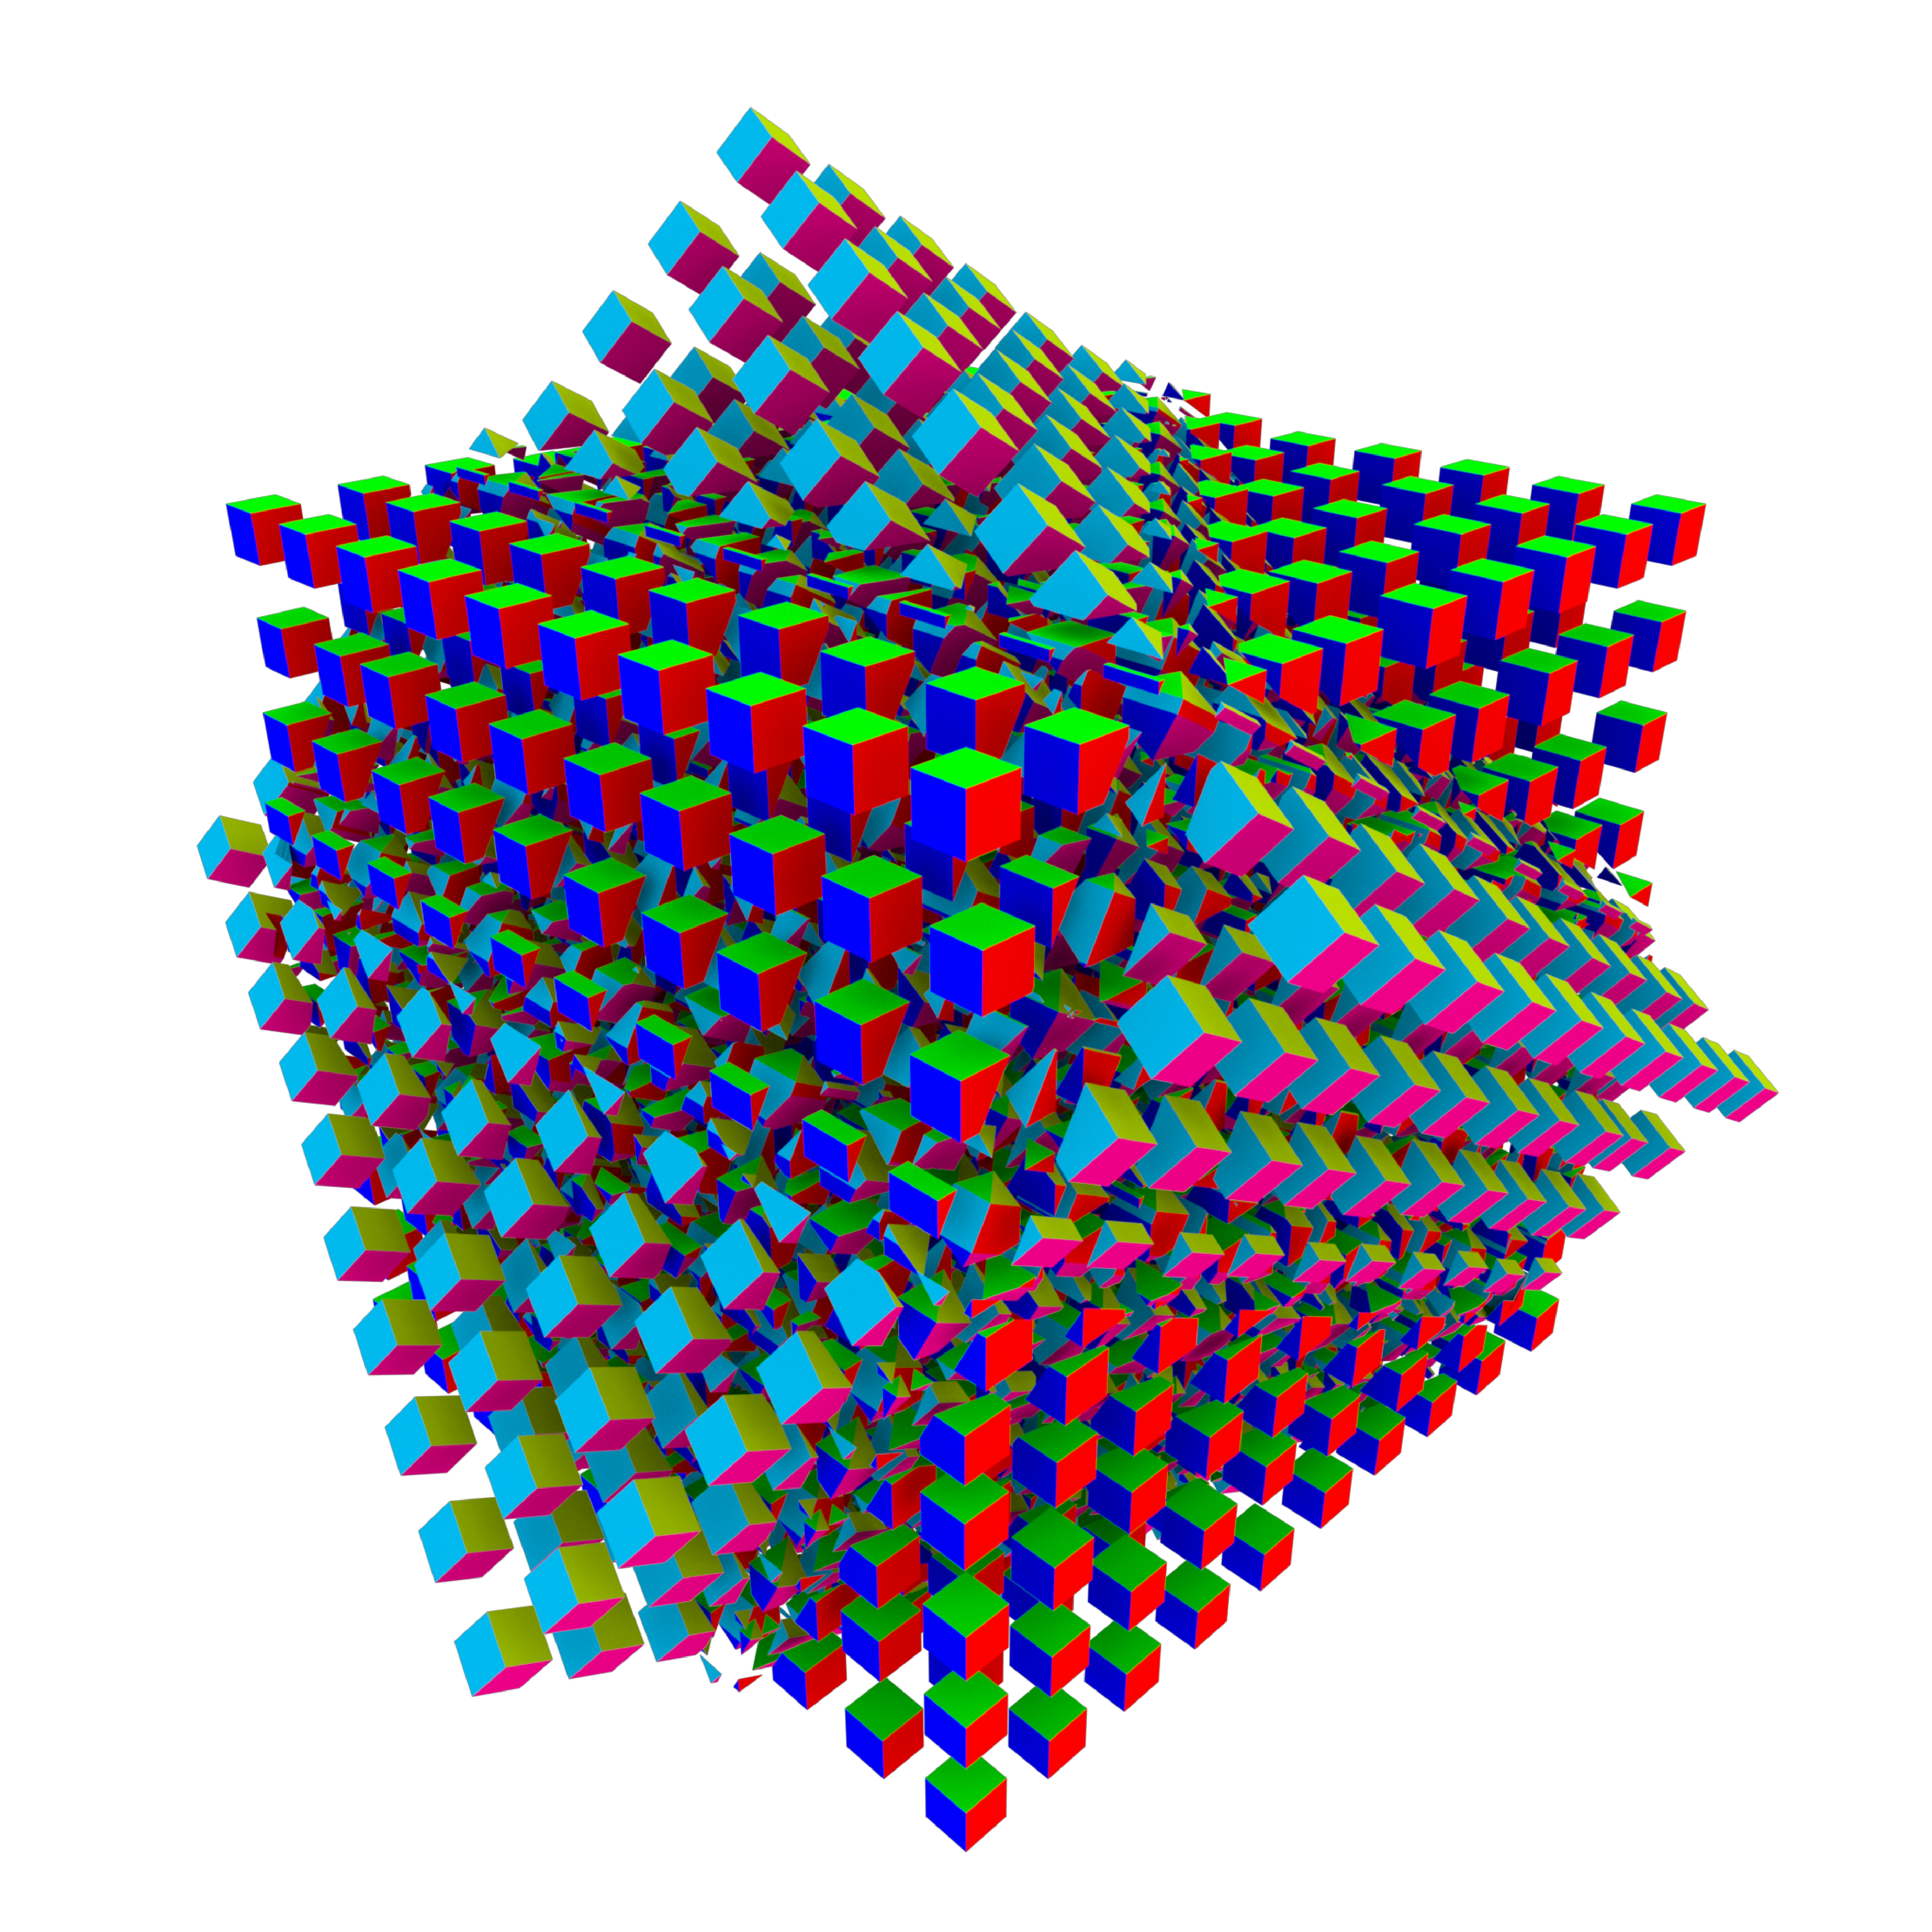
\includegraphics[width=\textwidth]{./img/cube10x10.pdf}
    \caption{Arrangement of 2000($=2\times10\times10\times10$) cubes}
\end{figure}





\section{Overview}
\label{sec:spatial_arrangement_overview}
The algorithm is based on the concept of recursive problem simplification 
(a sort of \textit{divide et impera} philosophy); if we have a $d$-complex, for every
($d-1$)-cell embedded into the $\mathbb{E}^d$ euclidean space, we bring the cell,
and every other cell that could intersect it, down into $\mathbb{E}^{d-1}$. We do this until
we reach the $d=1$ in $\mathbb{E}^1$ case; in here, we fragment all the $1$-cells.
Then, we travel back to the original $d$-dimension, and, for each
dimensional step, we build correct complexes from cells provided by the 
fragmentation of the lower dimension. 

\begin{figure}[h]
    \begin{center}
        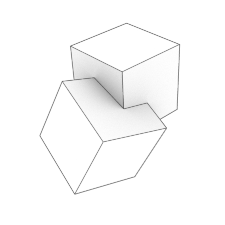
\includegraphics[width=.25\textwidth]{./img/ch1-1.pdf}%
        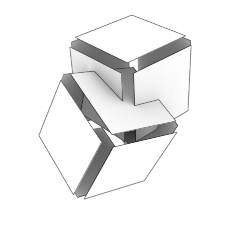
\includegraphics[width=.25\textwidth]{./img/ch1-2.pdf}%
        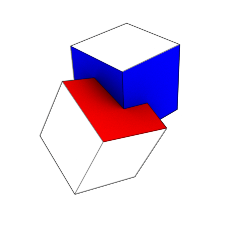
\includegraphics[width=.25\textwidth]{./img/ch1-3.pdf}%
        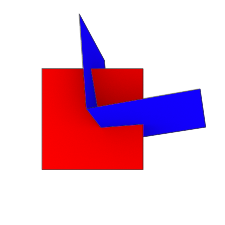
\includegraphics[width=.25\textwidth]{./img/ch1-4.pdf}%

        (a)\hspace{.22\textwidth}(b)\hspace{.22\textwidth}(c)\hspace{.22\textwidth}(d)
    \end{center}
    
    \begin{center}
        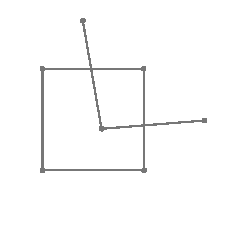
\includegraphics[width=.25\textwidth]{./img/ch1-5.pdf}%
        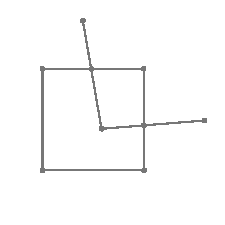
\includegraphics[width=.25\textwidth]{./img/ch1-6.pdf}%
        
\includegraphics[width=.25\textwidth]{./img/ch1-7.pdf}%
        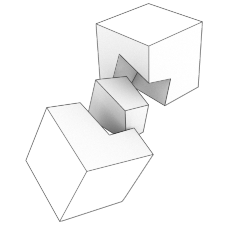
\includegraphics[width=.25\textwidth]{./img/ch1-8.pdf}%

        (e)\hspace{.22\textwidth}(f)\hspace{.22\textwidth}(g)\hspace{.22\textwidth}(h)
    \end{center}
    \caption{Algorithm overview}
    \label{img:spatial}
\end{figure}

We have in input two cellular complexes [fig. \ref{img:spatial}, a], 
given as 2-skeletons, which are the sets of 2-cells 
[fig. \ref{img:spatial}, b, exploded]. Once we merged the skeletons
[ref. \ref{sec:skel_merge}], we individuate for each $2$-cell (that we will call $\sigma$)
all the other cells that could intersect it. We do this by computing
the spatial index: it is a mapping $\mathcal{I}(\sigma)$ from a cell $\sigma$ to every other 
cell $\tau$ of which $box(\sigma) \cap box(\tau) \neq \emptyset$, where 
the $box$ function provides the axis aligned bounding box (AABB) of a cell [fig. \ref{img:spatial}, c, 
$\sigma$ in red and $\mathcal{I}(\sigma)$ in blue]. The spatial arrangement
calculation is speeded up by storing the AABBs as dimensional wise intervals
into an interval tree \cite{interval_trees}. 
Now for each cell $\sigma$ we transform $\sigma \cup \mathcal{I}(\sigma)$ 
in a way that $\sigma$ lays on the $x_3=0$ plane [fig. \ref{img:spatial}, d] and we find the intersections 
of the $\mathcal{I}(\sigma)$ cells with $x_3=0$ plane. So we have a ``soup''
of 1-cells in $\mathbb{E}^2$ [fig. \ref{img:spatial}, e], and we fragment each 1-cell 
with every other cell obtaining a valid 1-skeleton [fig. \ref{img:spatial}, f].
From this data it is possible to build the 2-cells using the ALGORITHM 1
presented and explored by Paoluzzi et al. \cite{Paoluzzi}
[fig. \ref{img:spatial}, g, exploded]. The procedure to fragment 1-cells
on a plane and return a 2-complex is called \textit{planar arrangement} and it
is presented more in detail in the next section. When the planar arrangement is
complete, fragmented $\sigma$ can be transformed back to its original position
in $\mathbb{E}^3$. With every 2-cell correctly fragmented, we can use the 
already cited ALGORITHM 1 again to build a full 3-complex%
\footnote{This is possible because ALGORITHM 1 is (almost) dimension independent
[ref. \ref{ch:minimal_cycles}].} [fig. \ref{img:spatial}, h, exploded].


\section{The ``$1$-cells in $\mathbb{E}^2$'' base case}
\label{sec:planar_arrangement_overview}

\begin{figure}[h]
    \centering
    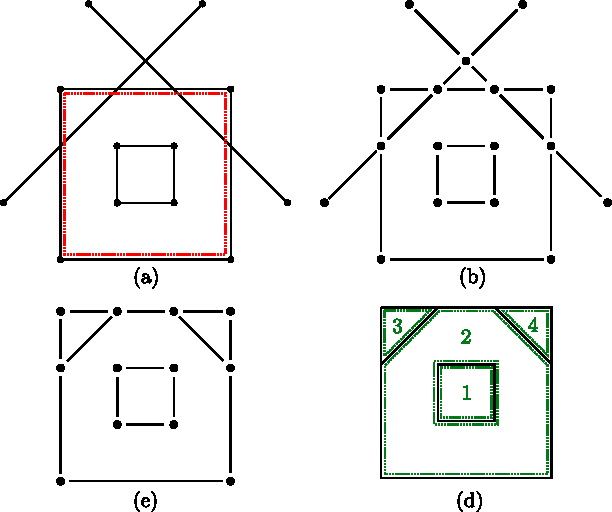
\includegraphics{./img/ch2-planararrangement.pdf}
    \caption{Planar arrangement overview}
    \label{img:planar}
\end{figure}

This is our base case. We have called \textit{planar arrangement} 
the procedure to handle this case since
it literally arranges a bunch of edges laying on a plane.
So, in input there are 1-cells in $\mathbb{E}^2$ and, optionally (but very
likely), the boundary of the original 2-cell $\sigma$ 
[fig. \ref{img:planar}, a, $\sigma$ in red].
We consider each edge and we fragment it with every other edge. This brings to
the creation of several coincident vertices: these will be eliminated
using a KD-Tree [fig. \ref{img:planar}, b, exploded]. 
At this point we have a perfectly fragmented 1-complex but many
edges are superfluous and must be eliminated; two kind of edges
are to discard: the ones outside the area of $\sigma$ and the ones
which are not part of a maximal biconnected component 
[ref. \ref{sec:biconnected_components}].
The result of this edge pruning outputs a
1-skeleton [fig. \ref{img:planar}, c, exploded].

After this, 2-cells must be computed:
for each connected component%
\footnote{It is legit to talk about a 1-skeleton as a graph: 
0-cells are nodes, 1-cells are edges and the boundary operator is
a incidence matrix.} we build a containment tree, which indicates
which component is spatially inside an other component.
Computing these relations, let us launch the ALGORITHM 1 \cite{Paoluzzi}
on each component and then combine the results to create 2-cells with non-intersecting 
shells\footnote{A 2-cell with a non-intersecting shell can be trivially defined
as a ``face with holes''; the correct definition is that it cannot 
be shrunk to the dimension of a point.} 
[fig. \ref{img:planar}, d, 2-cells numbered in green; please note that
cell 2 has cell 1 as an hole].


\section{Implementation}

Our implementation of this algorithm does not go over
$d=3$. It has been split in
multiple chapters in this book:

\begin{itemize}[noitemsep]
    \item Spatial Arrangement [ch. \ref{ch:spatial_arrangement}]: 
        It is the implementation of the ``$1$-cells in $\mathbb{E}^2$'' base case.
    \item Planar Arrangement [ch. \ref{ch:planar_arrangement}]:
        This treats the $d=3$ case. 
    \item Dimension travel [ch. \ref{ch:dimension_travel}]:
        Here are contained the utilities to travel from a
        dimension to another.
    \item Minimal cycles computation [ch. \ref{ch:minimal_cycles}]:
        This is dedicated to the implementation of the ALGORITHM 1
        described by Paoluzzi et Al. \cite{Paoluzzi}.
\end{itemize}

\part{Implementation}

\chapter{Module overview}



%===============================================================================
\section{Data transforms and boundary operators}\label{sec:boundary}
%===============================================================================

In this section we provide some Julia functions to compute (boundary) operator representations starting from other data representations, i.e., generally speaking, starting from one/two incidence relations.

\paragraph{Sparse characteristic matrices $M_p$}

The generic function \texttt{characteristicMatrix} produces a compressed sparse column representation of a single incidence relation, i.e.~the associated characteristic matrix $M_p$ In this code we use $p=2$ and \texttt{FV} as parameter name, but it may refer to any other incidence relation as actual value. The function employs a COO (coordinate) method to build the sparse matrix, i.e.~starts from a triple of arrays for \texttt{I,J,V} values.


%-------------------------------------------------------------------------------
@D Computation of sparse characteristic matrices $M_p$
@{
# Characteristic matrix $M_2$, i.e. M(FV)
function characteristicMatrix(FV)
	I,J,V = Int64[],Int64[],Int8[] 
	for f=1:length(FV)
		for k in FV[f]
			push!(I,f)
			push!(J,k)
			push!(V,1)
		end
	end
	M_2 = sparse(I,J,V)
	return M_2
end
@}
%-------------------------------------------------------------------------------


Hence we get the sparse matrix \texttt{cscEV}, shown in Figure~\ref{fig:intro-0}, by 
{\small\begin{verbatim}
cscEV = characteristicMatrix(EV)
\end{verbatim}}

\paragraph{Boundary matrix $[\partial_1] = [\delta_0]^\top$}

It is worth noting that the matrix $M_1=\texttt{cscEV}$ previously computed is very similar to the operator matrix $[\delta_0]$, but with elements in $\{-1,0,1\}$ instead than in $\{0,1\}$. The computation is than easily done, by using the fact that the 1-cell is written as oriented 0-chains $\eta=\nu_k - \nu_h$, with $k>h$, and hence in coordinates we have $\texttt{spboundary1}[k,e] = 1$ and $\texttt{spboundary1}[k,e] = -1$.

%-------------------------------------------------------------------------------
@D Computation of (signed) sparse boundary $C_1 \to C_0$
@{
# Computation of sparse boundary $C_1 \to C_0$
function boundary1(EV)
	spboundary1 = LARLIB.characteristicMatrix(EV)'
	for e = 1:length(EV)
		spboundary1[EV[e][1],e] = -1
	end
	return spboundary1
end
@}
%-------------------------------------------------------------------------------

In this case we get the compressed sparse column matrix representation $\partial_1$, shown dense in Figure~\ref{fig:intro-2}, by computing
\[
\partial_1 = \small\texttt{LARLIB.boundary1(EV)}
\]
\begin{figure}[htbp] %  figure placement: here, top, bottom, or page
{\footnotesize\begin{verbatim}
julia> julia> full(LARLIB.boundary1(EV))
12�20 Array{Int8,2}:
 -1   0   0   0   0   0  -1   0   0   0   0   0  -1   0   0   0   0   0   0   0
  1   0   0   0   0   0   0  -1   0   0   0   0   0  -1   0   0   0   0   0   0
  0  -1   0   0   0   0   1   0   0   0   0   0   0   0  -1   0   0   0   0   0
  0   1   0   0   0   0   0   1   0   0   0   0   0   0   0  -1   0   0   0   0
  0   0  -1   0   0   0   0   0  -1   0   0   0   1   0   0   0  -1   0   0   0
  0   0   1   0   0   0   0   0   0  -1   0   0   0   1   0   0   0  -1   0   0
  0   0   0  -1   0   0   0   0   1   0   0   0   0   0   1   0   0   0  -1   0
  0   0   0   1   0   0   0   0   0   1   0   0   0   0   0   1   0   0   0  -1
  0   0   0   0  -1   0   0   0   0   0  -1   0   0   0   0   0   1   0   0   0
  0   0   0   0   1   0   0   0   0   0   0  -1   0   0   0   0   0   1   0   0
  0   0   0   0   0  -1   0   0   0   0   1   0   0   0   0   0   0   0   1   0
  0   0   0   0   0   1   0   0   0   0   0   1   0   0   0   0   0   0   0   1
\end{verbatim}}
   \caption{Dense signed $[\partial_1]$ matrix $\partial_1$ for the small complex in Figure~\ref{fig:intro-1}}
   \label{fig:intro-2}
\end{figure}


\paragraph{Boundary matrix $[\partial_2] = [\delta_1]^\top$}

The matrix of the unsigned operator $\partial_2$ is computed here, according to the method introduced in~\cite{}. In particular, the two sparse incidence matrices \texttt{cscFV} and \texttt{cscEV} are first computed, and the product matrix in \texttt{temp} codifies, for any pair $(i,j)$ of indices the number of vertices shared between the  $i$-th 2-cell and the $j$-th 1-cell; when this number is equal to 2, the $j$-th 1-cell belongs to the boundary of the $i$-th 2-cell, so providing a triple $(i,j,1)$ to be inserted in the COO representation of \texttt{sp\_uboundary2}, and finally in its CSC representation.

%-------------------------------------------------------------------------------
@D Computation of (unsigned) sparse boundary $C_2 \to C_1$
@{
# Computation of sparse uboundary2
function uboundary2(FV,EV)
	cscFV = characteristicMatrix(FV)
	cscEV = characteristicMatrix(EV)
	temp = cscFV * cscEV'
	I,J,V = Int64[],Int64[],Int8[]
	for j=1:size(temp,2)
		for i=1:size(temp,1)
			if temp[i,j] == 2
    			push!(I,i)
    			push!(J,j)
    			push!(V,1)
			end
		end
	end
	sp_uboundary2 = sparse(I,J,V)
	return sp_uboundary2
end
@}
%-------------------------------------------------------------------------------


\paragraph{Signed boundary matrix $[\partial_2] = [\delta_1]^\top$}

Here we build a possible value for $[\partial_2] \in \{-1,0,1\}^m_n$. By rows, it describes each elementary 2-chain (2-cell) as a signed 1-cycle (1-chain without boundary). Since no standard orientation exists for $p$-cycles in $d$-space ($p < d$),
\emph{by convention} we compute each 1-cycle oriented as its first 1-cell, i.e. going in the direction from the second to the first 0-cell of it.

The construction algorithm may be split into two phases: the initialization and the loop indexed on faces. In turn, the faces loop calls the function \texttt{columninfo(col)}, deputed to store a quadruple of data providing a data structure to set properly (in sign) each 1-cell of a 1-cycle.

\subparagraph{Initialization}
%-------------------------------------------------------------------------------
@D Initialization of the (signed) sparse boundary
@{
# Initialization
function boundary2(FV,EV)
    sp_u_boundary2 = LARLIB.uboundary2(FV,EV)
    larEV = LARLIB.characteristicMatrix(EV)
    # unsigned incidence relation
    FE = [findn(sp_u_boundary2[f,:]) for f=1:size(sp_u_boundary2,1) ]
    I,J,V = Int64[],Int64[],Int8[]
    vedges = [findn(larEV[:,v]) for v=1:size(larEV,2)]
@}
%-------------------------------------------------------------------------------

\subparagraph{Local storage}
A local function \texttt{columninfo} is used to store the needed data structure into a temporary array \texttt{infos}

%-------------------------------------------------------------------------------
@D Local temporary storage function
@{
# Local storage
function columninfo(infos,EV,next,col)
    infos[1,col] = 1
    infos[2,col] = next
    infos[3,col] = EV[next][1]
    infos[4,col] = EV[next][2]
    vpivot = infos[4,col]
end
@}
%-------------------------------------------------------------------------------

\subparagraph{Loop on faces}
%-------------------------------------------------------------------------------
@D Loop on faces to construct the (signed) sparse boundary2
@{# Loop on faces
for f=1:length(FE)
    fedges = Set(FE[f])
    next = pop!(fedges)
    col = 1
    infos = zeros(Int64,(4,length(FE[f])))
    vpivot = infos[4,col]
    vpivot = columninfo(infos,EV,next,col)
    while fedges != Set()
        nextedge = intersect(fedges, Set(vedges[vpivot]))
        fedges = setdiff(fedges,nextedge)
        next = pop!(nextedge)
        col += 1
        vpivot = columninfo(infos,EV,next,col)
        if vpivot == infos[4,col-1]
            infos[3,col],infos[4,col] = infos[4,col],infos[3,col]
            infos[1,col] = -1
            vpivot = infos[4,col]
        end
    end
    for j=1:size(infos,2)
        push!(I, f)
        push!(J, infos[2,j])
        push!(V, infos[1,j])
    end
end
@}
%-------------------------------------------------------------------------------

The assembly of the whole function \texttt{boundary2(FV,EV)} is given below.

\subparagraph{Assembly signed boundary construction}

%-------------------------------------------------------------------------------
@D Computation of (signed) sparse boundary $C_2 \to C_1$
@{
@< Local temporary storage function @>
@< Initialization of the (signed) sparse boundary @>
    @< Loop on faces to construct the (signed) sparse boundary2 @>
    spboundary2 = sparse(I,J,V)
    return spboundary2
end
@}
%-------------------------------------------------------------------------------

%===============================================================================
\section{Chain complex construction}\label{sec:chaincomplex}
%===============================================================================
In this section we introduce the main function used to construct the chain complex of a space arrangement starting from a LAR input that may contain one or more cellular complexes.
The input is a standard LAR model, i.e., a triple with vertex coordinates, and incidennce realtions of 2-cells and 1-cells with vertices.
The output is a triple made by new \emph{vertices}, the new \emph{bases} for 1-, 2-, and 3-cells, and the signed boundary operators $\partial_1, \partial_2, \partial_3$.
%-------------------------------------------------------------------------------
@D Chain 3-complex construction
@{# Chain 3-complex construction
function chaincomplex(W,FW,EW)
    V = convert(Array{Float64,2},W')
    EV = characteristicMatrix(EW)
    FE = boundary2(FW,EW)
    V,cscEV,cscFE,cscCF = LARLIB.spatial_arrangement(V,EV,FE)
    ne,nv = size(cscEV)
    nf = size(cscFE,1)
    nc = size(cscCF,1)
    EV = [findn(cscEV[e,:]) for e=1:ne]
    FV = [collect(Set(vcat([EV[e] for e in findn(cscFE[f,:])]...)))  for f=1:nf]
    CV = [collect(Set(vcat([FV[f] for f in findn(cscCF[c,:])]...)))  for c=2:nc]
    function ord(cells)
        return [sort(cell) for cell in cells]
    end
    temp = copy(cscEV')
    for k=1:size(temp,2)
        h = findn(temp[:,k])[1]
        temp[h,k] = -1
    end    
    cscEV = temp'
    bases, coboundaries = (ord(EV),ord(FV),ord(CV)), (cscEV,cscFE,cscCF)
    return V',bases,coboundaries
end
@}
%-------------------------------------------------------------------------------

\paragraph{Collect one or more LAR models in a single model}

The goal of the function \texttt{collection2model} is to store a collection of LAR models (i.e.~triples (W,FW,EW)) into a single LAR model, by concatenation of vertex arrays, and concatenation of incidence relations, properly shifted.
The input type is \texttt{Array{Array{Array,1},1}}, the output type is \texttt{Tuple{Array{Float64,2},Array{Array{Int64,1},1},Array{Array{Int64,1},1}}}.
Of course, the result may not be the LAR representation of a cellular complex, since some cells may intersect out of boundaries.
Actually, this function prepares the input to be submitted to the \texttt{chaincomplex} function, that provides to mutually intersect the 2-cells and to reconstruct the 3-cells using the topological gift-wrapping algorithm~\cite{DBLP:journals/corr/PaoluzziSD17}.

%-------------------------------------------------------------------------------
@D Collect LAR models in a single LAR model
@{# Collect LAR models in a single LAR model
function collection2model(collection)
	W,FW,EW = collection[1]
	shiftV = size(W,2)
	for k=2:length(collection)
		V,FV,EV = collection[k]
		W = [W V]
		FW = [FW; FV + shiftV]
		EW = [EW; EV + shiftV]
		shiftV = size(W,2)
	end
	return W,FW,EW
end
@}
%-------------------------------------------------------------------------------

\paragraph{Triangulation of a single 2-cell embedded in 3D}

The 2-cells of a LAR cellular complex may have any kind of geometry or topology, provided they are connected. In other words, the 2-cells may be either convex or no-convex, and either simply connected or multiply connected, i.e.~containing any finite number of internal holes. Of course, the topological gift-wrapping algorithm~cite{DBLP:journals/corr/PaoluzziSD17}, introduced to extract the basis of 3-cells as minimal cycles of 2-cells,
has no problems in handling such general kind of 2-cells. Conversely, in order to draw the complex, or to show its shape into an interactive viewer, a decomposition of the boundary of every 3-cell into a set of triangles (triple of 3-points) is needed, since this one is the only data structure accepted by the graphics hardware.

The following higher-level function \texttt{facetriangulation} computes this triangulation for the generic 2-cell indexed by \texttt{f}, taking as input (for the first application) also the vertices \texttt{V}, the incidence relation \texttt{FV}, and the coboundary operators $\delta_1$ and $\delta_2$. In particular, for each 2-cell $f$, a \emph{local} LAR representation \texttt{vts} is generated using a vertex dictionary \texttt{vdict} and its inverse map \texttt{dictv}. The 2-face is trasformed in the 2-subspace $z=0$ using the transformation matrix \texttt{inv(M)}, in order to prepare the types of data expected by the \texttt{TRIANGLE.constrained\_triangulation\_vertices} that performs a CDT (Constrained Delaunay Triangulation) algorithm so finally returning the incidence relation between triangle and (original) vertices named \texttt{mktriangles}.

%-------------------------------------------------------------------------------
@D Triangulation of a single facet
@{# Triangulation of a single facet
function facetriangulation(V,FV,EV,cscFE,cscCF)
	function facetrias(f)
		vs = [V[:,v] for v in FV[f]]
		vs_indices = [v for v in FV[f]]
		vdict = Dict([(i,index) for (i,index) in enumerate(vs_indices)])
		dictv = Dict([(index,i) for (i,index) in enumerate(vs_indices)])
		es = findn(cscFE[f,:])
	
		vts = [v-vs[1] for v in vs]
	
		v1 = vts[2]
		v2 = vts[3]
		v3 = cross(v1,v2)
		err, i = 1e-8, 1
		while norm(v3) < err
			v2 = vts[3+i]
			i += 1
			v3 = cross(v1,v2)
		end	
	
		M = [v1 v2 v3]

		vs_2D = hcat([(inv(M)*v)[1:2] for v in vts]...)'
		pointdict = Dict([(vs_2D[k,:],k) for k=1:size(vs_2D,1)])
		edges = hcat([[dictv[v] for v in EV[e]]  for e in es]...)'
	
		trias = TRIANGLE.constrained_triangulation_vertices(
			vs_2D, collect(1:length(vs)), edges)

		triangles = [[pointdict[t[1,:]],pointdict[t[2,:]],pointdict[t[3,:]]] 
			for t in trias]
		mktriangles = [[vdict[t[1]],vdict[t[2]],vdict[t[3]]] for t in triangles]
		return mktriangles
	end
	return facetrias
end
@}
%-------------------------------------------------------------------------------

\paragraph{Triangulation of the whole 2-skeleton}

The \texttt{cf} tuple, that constitute the main input of the \texttt{triangulate} function, contains the COO representation of the signed sparse matrix $[\delta_2]$.
The aim of \texttt{triangulate} is to produce the incidence relation \texttt{TV} between the oriented triangles \texttt{T} and the vertices \texttt{V} of the 3-skeleton of our cellular complex.

%-------------------------------------------------------------------------------
@D Triangulation of the 2-skeleton
@{# Triangulation of the 2-skeleton
function triangulate(cf,V,FV,EV,cscFE,cscCF)
	mktriangles = LARLIB.facetriangulation(V,FV,EV,cscFE,cscCF)
	TV = Array{Int64,1}[]
	for (f,sign) in zip(cf[1],cf[2])
		triangles = mktriangles(f)
		if sign == 1
			append!(TV,triangles )
		elseif sign == -1
			append!(TV,[[t[2],t[1],t[3]] for t in triangles] )
		end
	end
	return TV
end
@}
%-------------------------------------------------------------------------------

\paragraph{Map 3-cells to local 2-chain bases}

%-------------------------------------------------------------------------------
@D Map 3-cells to local bases
@{# Map 3-cells to local bases
function map_3cells_to_localbases(V,CV,FV,EV,cscCF,cscFE)
	local3cells = []
	for c=1:length(CV)
		cf = findnz(cscCF[c+1,:])
		tv = LARLIB.triangulate(cf,V,FV,EV,cscFE,cscCF)
		vs = sort(collect(Set(hcat(tv...))))
		vsdict = Dict([(v,k) for (k,v) in enumerate(vs)])
		tvs = [[vsdict[t[1]],vsdict[t[2]],vsdict[t[3]]] for t in tv]
		v = hcat([V[:,w] for w in vs]...)
		cell = [v,tvs]
		append!(local3cells,[cell])
	end
	return local3cells
end
@}
%-------------------------------------------------------------------------------

\paragraph{Visualize solid (explosed) cells}

%-------------------------------------------------------------------------------
@D Visualize solid cells
@{# Visualize solid cells
function viewsolidcells(sx=1.2, sy=1.2, sz=1.2)
	scaling = [sx; sy; sz]
	function viewsolidcells0(V,CV,FV,EV,cscCF,cscFE)
		local3cells = LARLIB.map_3cells_to_localbases(V,CV,FV,EV,cscCF,cscFE)
		hpcs = Any[]
		for local3cell in local3cells
			v,tv = local3cell
			centroid = sum(v,2)/size(v,2)
			scaledcentroid = scaling.*centroid
			translation = scaledcentroid - centroid
			w = v .+ translation
			hpc = p.SOLIDIFY(LARVIEW.lar2hpc(w,tv))
			append!(hpcs, [hpc])
		end
		p.VIEW(p.STRUCT(hpcs))
		return viewsolidcells0
	end
end
@}
%-------------------------------------------------------------------------------



@O lib/jl/LARLIB.jl
@{module LARLIB

	@< LAR imports @>
	@< LAR types @>
	@< Computation of sparse characteristic matrices $M_p$ @>
	@< Computation of (signed) sparse boundary $C_1 \to C_0$ @>
	@< Computation of (unsigned) sparse boundary $C_2 \to C_1$ @>
	@< Computation of (signed) sparse boundary $C_2 \to C_1$ @>
	@< Chain 3-complex construction @>
	@< Collect LAR models in a single LAR model @>
	@< Triangulation of a single facet @>
	@< Triangulation of the 2-skeleton @>
	@< Map 3-cells to local bases @>
	@< Visualize solid cells @>

	include("./utilities.jl")
	include("./minimal_cycles.jl")
	include("./dimension_travel.jl")
	include("./planar_arrangement.jl")
	include("./spatial_arrangement.jl")
	include("./largrid.jl")
	
end
@}

%%%%%%%%%%%%%%%
\section{Standard types}

We define at the top of our module the standard types
that will be used throughout LAR. As already explained
in the introduction [ref. \ref{sec:LAR}], LAR needs
only one bi-dimensional array to store geometry and 
one or more sparse matrices for topology.
Julia has already implemented CSC sparse matrices in
its standard library so we are going to use them.

@D LAR types
@{const Verts = Array{Float64, 2}
const Cells = SparseMatrixCSC{Int8, Int}
const Cell = SparseVector{Int8, Int}
const LarCells = Array{Array{Int, 1}, 1}
@}

We used the general name \texttt{Cells}, but
we are going to use this type also for boundaries.

\subsection{Floating point error}
\label{sec:floating-point_error}

We stored geometry using 64-bit IEEE floats.
As it is known, floating point arithmetic is not
precise and introduces numerical errors.
Usually this is not an issue\footnote{The \textit{machine epsilon},
which is the upper bound on the relative error in floating-point 
arithmetic, for double precision IEEE floating-point numbers is 
$2^53 \approx 1.11 \times 10^{-16}$.}, but when precision is
a goal, floating point error must be handled very carefully.
During the development we encountered several numerical problems
and we tried various approaches (like normalizing the geometry
inside the $[0, 1]$ interval for each dimension in order to maximize
the significand of the floating-point numbers) but most of them turned 
out to be unstable. So we choose the less orthodox path we could
possibly take: we set a fixed error and we performed every floating point
comparison using this error. Examples of this ``tweak'' are to be found in
\ref{sec:intersect_edges}, \ref{sec:face_int}, \ref{sec:3d_minimal_cycles} and 
\ref{sec:vertex_equality}.

%%%%%%%%%%%%%%%%%
\section{Notes on variables names}

Here a list of some often used variable names.

\begin{description}[align=right,labelwidth=2em]
    \item [\texttt{V}:]
        Bi-dimensional array (\texttt{Verts}) that keeps the geometry of a complex.
        Its dimensions are $n \times d$, where $n$ is the number of vertices and $d$ is the dimension
        of the euclidean space in which the complex is embedded.
    \item [\texttt{EV}:]
        1-boundary. It is a $m \times n$ sparse matrix (\texttt{Cells}) 
        where $m$ is the number of edges and $n$ is the number of vertices. The possible values
        are $0, 1$ and $-1$.
    \item [\texttt{FE}:]
        2-boundary. Same as \texttt{EV}, but faces on the rows and edges on the columns.
    \item [\texttt{CF}:]
        3-boundary. Same as \texttt{EV}, but 3-cells on the rows and faces on the columns.
\end{description}

%%%%%%%%%%%%%%%
\section{Tests and examples}

There are several unit tests throughout the implementation. They
are inside the \texttt{test} directory and can be run at once
by executing \texttt{test/runtests.jl}

@O test/jl/runtests.jl
@{using LARLIB

include("./planar_arrangement.jl")
include("./dimension_travel.jl")
include("./largrid.jl")
include("./utilities.jl")
@}

%--------------------------------------------------------------------------------
\subsection{Unit tests on LARLIB.jl}
%--------------------------------------------------------------------------------

%-------------------------------------------------------------------------------
@O test/jl/larlib.jl
@{
@@testset "Boundary operators Tests" begin
   @@testset "characteristicMatrix" begin
      V,cells = LARLIB.larCuboids([2,1,1],true) 
      VV,EV,FV,CV = cells
      @@test typeof(V)==Array{Float64,2}
      @@test typeof(cells)==Array{Array{Array{Int64,1},1},1}
      @@testset "$rel" for rel in cells
         @@test typeof(rel)==Array{Array{Int64,1},1}
         @@test typeof(LARLIB.characteristicMatrix(rel))==SparseMatrixCSC{Int8,Int64}
      end
   end

   @@testset "boundary1 Tests" begin
      V,cells = LARLIB.larCuboids([2,1,1],true) 
      VV,EV,FV,CV = cells
      @@testset "$rel" for rel in cells
         @@test typeof(rel)==Array{Array{Int64,1},1}
         @@test typeof(LARLIB.boundary1(rel))==SparseMatrixCSC{Int8,Int64}
         @@test size(LARLIB.boundary1(EV))==(size(V,2),length(EV)) 
      end
   end

   @@testset "uboundary2 Tests" begin
      V,cells = LARLIB.larCuboids([2,1,1],true) 
      VV,EV,FV,CV = cells
      @@test typeof(LARLIB.uboundary2(FV,EV))==SparseMatrixCSC{Int8,Int64}
      @@test size(LARLIB.uboundary2(FV,EV))==(length(FV),length(EV)) 
   end

   @@testset "boundary2 Tests" begin
      V,cells = LARLIB.larCuboids([2,1,1],true) 
      VV,EV,FV,CV = cells
      @@test typeof(LARLIB.boundary2(FV,EV))==SparseMatrixCSC{Int8,Int64}
      @@test size(LARLIB.boundary2(FV,EV))==(length(FV),length(EV)) 
      @@test sum(findnz(LARLIB.boundary2(FV,EV))[3])==0
   end

   @@testset "chaincomplex Tests" begin
      V,cells = LARLIB.larCuboids([2,1,1],true) 
      VV,EV,FV,CV = cells
      bases,coboundaries = LARLIB.chaincomplex(V,FV,EV)[2:3]
      @@test typeof(bases)==Tuple{Array{Array{Int64,1},1},Array{Array{Int64,1},1},
         Array{Array{Int64,1},1}}
      @@test typeof(coboundaries)==Tuple{SparseMatrixCSC{Int8,Int64},
         SparseMatrixCSC{Int8,Int64},SparseMatrixCSC{Int8,Int64}}
      @@testset "$basis" for basis in bases
         @@test typeof(basis)==Array{Array{Int64,1},1}
      end
      @@testset "$coboundary" for coboundary in coboundaries
         @@test typeof(coboundary)==SparseMatrixCSC{Int8,Int64}
      end
   end
   
   @@testset "collection2model Tests" begin
      @@test typeof(collection)==Array{Array{Array,1},1}
   end

   @@testset "facetriangulation Tests" begin
      V,(VV,EV,FV,CV) = LARLIB.larCuboids([2,2,1],true)
      W,FW,EW = copy(V),copy(FV),copy(EV)
      collection = Array{Array,1}[]
      for k=1:2
    	 W,FW,EW = copy(W)+.5,copy(FV),copy(EV)
    	 append!(collection, [[W,FV,EV]])
      end
      V,FV,EV = LARLIB.collection2model(collection)
      V,bases,coboundaries = LARLIB.chaincomplex(V,FV,EV)
      EV,FV,CV = bases
      cscEV,cscFE,cscCF = coboundaries
      TV = triangulate((1:length(FV),ones(length(FV))),V,FV,cscFE,cscCF)
      @@test typeof(TV)==Array{Array{Int64,1},1}
      @@test typeof((V,FV))==Tuple{Array{Float64,2},Array{Array{Int64,1},1}}
      @@test typeof((1:length(FV),ones(length(FV))))==Tuple{UnitRange{Int64},Array{Float64,1}}
      @@testset "$triangle" for triangle in TV
         @@test length(triangle)==3
      end
   end
end
@}
%-------------------------------------------------------------------------------




Also general examples of some main functionalities are provided.
They can be found into \texttt{examples/general\_examples.jl}

@O examples/jl/general_examples.jl
@{using LARLIB

@< planar\_arrangement general examples @>
@< spatial\_arrangement general examples @>
@}
\chapter{Spatial Arrangement}

%%%%%%%%%%%%%%%%%%
\section{Overview}
Here we present the spatial arrangement algorithm.
It has been explained in the introduction [ref. \ref{sec:spatial_arrangement_overview}].

@O lib/jl/spatial_arrangement.jl
@{@< spatial\_arrangement support functions @>

function spatial_arrangement(V::Verts, EV::Cells, FE::Cells)
    vs_num = size(V, 1)
    es_num = size(EV, 1)
    fs_num = size(FE, 1)

    sp_idx = spatial_index(V, EV, FE)

    rV = Verts(0,3)
    rEV = spzeros(Int8,0,0)
    rFE = spzeros(Int8,0,0)

    for sigma in 1:fs_num
        println(sigma, "/", fs_num)

        sigmavs = (abs.(FE[sigma:sigma,:])*abs.(EV))[1,:].nzind 
        sV = V[sigmavs, :]
        sEV = EV[FE[sigma, :].nzind, sigmavs]

        @< Sigma flattening @>

        nV, nEV, nFE = planar_arrangement(sV, sEV, sparsevec(ones(Int8, length(sigmavs))))

        if nV == nothing
            continue
        end
        
        nvsize = size(nV, 1)
        nV = [nV zeros(nvsize) ones(nvsize)]*inv(M)[:, 1:3]

        rV, rEV, rFE = skel_merge(rV, rEV, rFE, nV, nEV, nFE)
    end

    rV, rEV, rFE = merge_vertices(rV, rEV, rFE)

    @< Create 3-cells @>

    return rV, rEV, rFE, rCF
end

@}

To flatten the 2-cell $\sigma$ on the $x_3=0$ plane,
we build a linear transformation matrix with the
\texttt{submanifold\_mapping} utility [ref. \ref{sec:submanifold_mapping}],
we transform the geometry and we intersect every cell in $\mathcal{I}(\sigma)$
[ref. \ref{sec:spatial_arrangement_overview}]
with the $x_3=0$ plane using \texttt{face\_int} [ref. \ref{sec:face_int}].

@D Sigma flattening
@{M = submanifold_mapping(sV)
tV = ([V ones(vs_num)]*M)[:, 1:3]

sV = tV[sigmavs, :]

for i in sp_idx[sigma]
    tmpV, tmpEV = face_int(tV, EV, FE[i, :])
    
    sV, sEV = skel_merge(sV, sEV, tmpV, tmpEV)
end

sV = sV[:, 1:2]
@}



%%%%%%%%%%%%%%%%%%%%%%%%%%%%%%%%%%%
\section{Coincident vertices merge}
\label{sec:3D_merge_vertices}

The merge of coincident is done in the \texttt{merge\_vertices}
function.

@D spatial\_arrangement support functions
@{function merge_vertices(V::Verts, EV::Cells, FE::Cells, err=1e-4)
    vertsnum = size(V, 1)
    edgenum = size(EV, 1)
    facenum = size(FE, 1)
    newverts = zeros(Int, vertsnum)
    kdtree = KDTree(V')

    @< Find coincident vertices @>
    @< Merge edges @>
    @< Merge faces @>

    return nV, nEV, nFE
end
@}

First of all we need to find vertices which are near enough
to be considered coincident. We perform this operation
relying on the \texttt{NearestNeighbors.jl} package\cite{NearestNeighbors}
which provides a rather good implementation of the \texttt{KDTree} data structure.

So, we identify the vertices to delete and we store a map
from original vertices to new vertices. In the meanwhile
we built a list of vertices to delete and we delete them 
as soon as possible.

@D LAR imports
@{using NearestNeighbors
@}

@D Find coincident vertices
@{todelete = []

i = 1
for vi in 1:vertsnum
    if !(vi in todelete)
        nearvs = inrange(kdtree, V[vi, :], err)

        newverts[nearvs] = i

        nearvs = setdiff(nearvs, vi)
        todelete = union(todelete, nearvs)

        i = i + 1
    end
end

nV = V[setdiff(collect(1:vertsnum), todelete), :]
@}

To delete the edges we write them as couples of vertex
indices. We keep them in two versions: in \texttt{edges}
we put the edges described with the indexes of the new vertices
and in \texttt{oedges} we put the edges relative to the original vertex
indices (we will use them when merging faces). Once we "translated"
the edges, we delete the duplicates (using a set union) and the
degenerated edges. Lastly we build a new EV matrix 
(called \texttt{nEV}). While we
build the matrix, we also build a dictionary which maps edges expressed
as couples of vertex indices into edge indices relative to \texttt{nEV};
this data will be used in the $d=2$ version of this function 
[ref. \ref{sec:2D_merge_vertices}].

@D Merge edges
@{edges = Array{Tuple{Int, Int}, 1}(edgenum)
oedges = Array{Tuple{Int, Int}, 1}(edgenum)

for ei in 1:edgenum
    v1, v2 = EV[ei, :].nzind
    
    edges[ei] = Tuple{Int, Int}(sort([newverts[v1], newverts[v2]]))
    oedges[ei] = Tuple{Int, Int}(sort([v1, v2]))

end
nedges = union(edges)
nedges = filter(t->t[1]!=t[2], nedges)

nedgenum = length(nedges)
nEV = spzeros(Int8, nedgenum, size(nV, 1))

etuple2idx = Dict{Tuple{Int, Int}, Int}()

for ei in 1:nedgenum
    nEV[ei, collect(nedges[ei])] = 1
    etuple2idx[nedges[ei]] = ei
end
@}

To merge the faces, we convert them into a lists of
edges (represented as a couple of vertices). We then remove duplicated faces
by checking which faces use the same vertices. At the end, we use the
maps built during vertices and edges merge to rebuild the \texttt{FE}
matrix correctly using the new vertex indices.

@D Merge faces
@{faces = [[
    map(x->newverts[x], FE[fi, ei] > 0 ? oedges[ei] : reverse(oedges[ei]))
    for ei in FE[fi, :].nzind
] for fi in 1:facenum]


visited = []
function filter_fn(face)

    verts = []
    map(e->verts = union(verts, collect(e)), face)
    verts = Set(verts)

    if !(verts in visited)
        push!(visited, verts)
        return true
    end
    return false
end

nfaces = filter(filter_fn, faces)

nfacenum = length(nfaces)
nFE = spzeros(Int8, nfacenum, size(nEV, 1))

for fi in 1:nfacenum
    for edge in nfaces[fi]
        ei = etuple2idx[Tuple{Int, Int}(sort(collect(edge)))]
        nFE[fi, ei] = sign(edge[2] - edge[1])
    end
end
@}




%%%%%%%%%%%%%%%%%%%%%%%%%%%%%%%%%%%
\section{$3$-cells creation}

@D Create 3-cells
@{@< Compute connected components @>
@< Compute containment tree @>
@< Cell union @>

rCF = minimal_3cycles(rV, rEV, rFE)
@}
\chapter{Planar Arrangement}
\label{ch:planar_arrangement}

%%%%%%%%%%%%%%%%%%
\section{Overview}
\label{sec:planar_arrangement_intro}

Refer to the introduction for algorithm explanation
[ref. \ref{ch:arrangement_algorithm}].
In the implementation we also build and return a 
map from the original edges to the new ones: this 
is necessary infrastructure to later implement
boolean operations with ease.

@O lib/jl/planar_arrangement.jl
@{using DataStructures
@< planar\_arrangement support functions @>

function frag_edge_channel(in_chan, out_chan)
    println("Worker[",myid(),"] - start")
    run_loop = true
    while run_loop
        # println("Worker[",myid(),"] - took a job")
        frag_job = take!(in_chan)
        id_job = frag_job[1]
        if id_job != -1
            V, EV, edgenum = frag_job[2]
            put!(out_chan, ( edgenum, (frag_edge(V, EV, edgenum )) ) )            
        else
            println("Worker[",myid(),"] - suicide")
            run_loop = false
        end
        # println("Worker[",myid(),"]- done a job")
    end
end

function planar_arrangement(V::Verts, EV::Cells, sigma::Cell=spzeros(Int8, 0), multiproc=true)
    edgenum = size(EV, 1)
    @< planar\_arrangement local variables @>

    in_chan = nothing
    out_chan = nothing


    if (multiproc == true)
        in_chan = RemoteChannel(()->Channel{Tuple}(0))
        out_chan = RemoteChannel(()->Channel{Tuple}(0))
    end
    
    if (multiproc == true)
        ordered_dict = SortedDict{Int64,Tuple}()

        @@schedule begin
            println("Sending data to channels ")
            for i in 1:edgenum
                put!(in_chan,(i,(V, EV, i)))
            end
            for p in workers()
                put!(in_chan,(-1,()))
            end
            println("Done sending data to channels")
        end

        for p in workers()
                println("Starting worker ", p)
                @@async Base.remote_do(frag_edge_channel, p, in_chan, out_chan)
        end

        println("Retrieving data from channels. Should be: ", edgenum)
        for i in 1:edgenum
            frag_done_job = take!(out_chan)
            ordered_dict[frag_done_job[1]] = frag_done_job[2]
        end
        println("Done retrieving data from channels. Got: ", length(ordered_dict) )

        println("Reassembling data")
        for (dkey, dval) in ordered_dict
            println("Reassembling data - ", dkey)
            i = dkey
            v, ev = dval
            newedges_nums = map(x->x+finalcells_num, collect(1:size(ev, 1)))
            
            edge_map[i] = newedges_nums
            
            finalcells_num += size(ev, 1)
            
            rV, rEV = skel_merge(rV, rEV, v, ev)
        end

        println("Done parallel")

    else
        for i in 1:edgenum
            v, ev = frag_edge(V, EV, i)
            
            newedges_nums = map(x->x+finalcells_num, collect(1:size(ev, 1)))
            
            edge_map[i] = newedges_nums
            
            finalcells_num += size(ev, 1)
            rV, rEV = skel_merge(rV, rEV, v, ev)
        end
    end
    
    V, EV = rV, rEV
    return V,EV

    @< Merge coincident vertices @>
    @< Delete edges outside sigma area @>
    @< Find maximal biconnected components @>
    @< Filter biconnected components @>
    @< Create faces @>  

    V, EV, FE, edge_map
end 
@}

The mapping from old edges to new ones is stored into \texttt{edge\_map}.

@D planar\_arrangement local variables
@{edge_map = Array{Array{Int, 1}, 1}(edgenum)
@}
%++++++++++++++++%
\subsection{Tests and examples}
Every function responsible for the planar arrangement is coupled by some tests. 
@O test/jl/planar_arrangement.jl
@{using Base.Test
using LARLIB

@< planar\_arrangement support functions tests @>
@}

Examples to show the functionalities implemented in this chapter
are defined at the end of it [ref. \ref{sec:planar_arrangement_examples}].










%%%%%%%%%%%%%%%%%%%%%%%%%%%%
\section{Edge fragmentation}
%+++++++++++++++++++++++++++%
\subsection{Support function}
\label{sec:frag_edge}
The edge fragmentation is performed by using a function called \texttt{frag\_edge}.
It fragments the edge of index \texttt{edge\_idx} computing the intersections of
it with the other edges of the complex. It returns the updated vertices list and the freshly computed edges.
For every edge, it needs to check if the edge to fragment intersects with it. 
The actual edge intersections are computed by \texttt{intersect\_edges} function [ref. \ref{sec:intersect_edges}]
The intersection points are then sorted along the edge to fragment, and correct fragments (which are edges themselves)
are computed.

@D planar\_arrangement support functions
@{function frag_edge(V::Verts, EV::Cells, edge_idx::Int)
    alphas = Dict{Float64, Int}()
    edge = EV[edge_idx, :]
    verts = V[edge.nzind, :]
    for i in 1:size(EV, 1)
        if i != edge_idx
            intersection = intersect_edges(V, edge, EV[i, :])
            for (point, alpha) in intersection
                verts = [verts; point]
                alphas[alpha] = size(verts, 1)
            end
        end
    end

    alphas[0.0], alphas[1.0] = [1, 2]

    alphas_keys = sort(collect(keys(alphas)))
    edge_num = length(alphas_keys)-1
    verts_num = size(verts, 1)
    ev = spzeros(Int8, edge_num, verts_num)

    for i in 1:edge_num
        ev[i, alphas[alphas_keys[i]]] = 1
        ev[i, alphas[alphas_keys[i+1]]] = 1
    end

    verts, ev
end
@}
%+++++++++++++++++++++++++++++%
\subsection{Edge intersections}
\label{sec:intersect_edges}
Three major cases are to be considered when intersecting two edges:
\begin{enumerate}[noitemsep]
    \item They are not parallel
    \item They are colinear (they stand on the same line) 
    \item They are parallel but not colinear
\end{enumerate}
In the third case there will be no intersections for sure so this case is skipped.
When they are not parallel there will be no more than a single intersection; in this case
we use the method presented by Bourke\cite{Bourke} to calculate it.
Particular attention is needed on the case of colinear edges: it can happen
that \texttt{edge2} is contained into the bounds of the colinear \texttt{edge1}; in this case, both points of
\texttt{edge2} are to be considered intersection and hence must be returned. Because of this, 
the intersections are returned as a list than can contain from zero to two elements; 
each element is a couple containing the intersection
point and a parameter useful for sorting the fragmentation points of an edge.

Here we are doing floating-point numbers comparisons so we use a fixed
error to avoid numerical imprecisions [ref. \ref{sec:floating-point_error}].

@D planar\_arrangement support functions
@{function intersect_edges(V::Verts, edge1::Cell, edge2::Cell)
    err = 10e-8

    x1, y1, x2, y2 = vcat(map(c->V[c, :], edge1.nzind)...)
    x3, y3, x4, y4 = vcat(map(c->V[c, :], edge2.nzind)...)
    ret = Array{Tuple{Verts, Float64}, 1}()

    v1 = [x2-x1, y2-y1];
    v2 = [x4-x3, y4-y3];
    v3 = [x3-x1, y3-y1];

    @< Check if colinear or parallel @>

    if colinear
        @< Handle colinear edges @>
    elseif !parallel
        denom = (v2[2])*(v1[1]) - (v2[1])*(v1[2])
        a = ((v2[1])*(-v3[2]) - (v2[2])*(-v3[1])) / denom
        b = ((v1[1])*(-v3[2]) - (v1[2])*(-v3[1])) / denom

        if -err < a < 1+err && -err <= b <= 1+err
            p = [(x1 + a*(x2-x1))  (y1 + a*(y2-y1))]
            push!(ret, (p, a)) 
        end
    end

    return ret
end
@}

To check if edges are parallel, we check with the dot product 
the parallelism between the edges defining vectors.
Edges are colinear if they are parallel and the points of
the second edge stand on the line of the first edge
or one of the points of the second edge is coincident to
one point of the first one.

@D Check if colinear or parallel
@{ang1 = dot(normalize(v1), normalize(v2))
ang2 = dot(normalize(v1), normalize(v3))

parallel = 1-err < abs(ang1) < 1+err
colinear = parallel && (1-err < abs(ang2) < 1+err || -err < norm(v3) < err)
@}

In the case of colinearity, 
to find if \texttt{edge2} has one or both of 
its vertices inside \texttt{edge1} we follow this procedure:
\begin{enumerate}
\item We parametrize \texttt{edge1}:
\[
    p = p_1 + \alpha(p_2-p_1), \quad\alpha\in[0, 1]
\]
Where $p_1$ and $p_2$ are the vertices of \texttt{edge1}
\item We solve for $\alpha$:
\begin{gather*}
    o = p_1, \quad\vec{v} = p_2 - p_1 \\
    p = o + \alpha\vec{v} \\
    p - o = \alpha\vec{v} \\
    \vec{v}^\top\cdot(p-o) = \alpha (\vec{v}^\top\cdot\vec{v}) \\
    \alpha = \frac{\vec{v}^\top\cdot(p-o)}{\vec{v}^\top\cdot\vec{v}}
\end{gather*}
\item We replace $p$ of the last equation with both the vertices of \texttt{edge2}.
If the result is $\in[0,1]$ then an intersection is found.
\end{enumerate} 
@D Handle colinear edges
@{o = [x1 y1] 
v = [x2 y2] - o
alpha = 1/dot(v,v')
ps = [x3 y3; x4 y4]
for i in 1:2
    a = alpha*dot(v',(reshape(ps[i, :], 1, 2)-o))
    if 0 < a < 1
        push!(ret, (ps[i:i, :], a))
    end
end
@}
%+++++++++++++++++++++++++%
\subsection{Implementation}

When we need to fragment an edge we just use the \texttt{frag\_edge} function [ref. \ref{sec:frag_edge}]
and we update data and store the changes.
While we fragment the edges, we also build a temporary version of \texttt{edge\_map}[ref. \ref{sec:planar_arrangement_intro}]. We do this using \texttt{i}
(the index of the edge that must be fragmented) and the indices of the new edges inside \texttt{ev}
offset by the \texttt{finalcells\_num} counter, which is updated at every step adding the numbers of
fragments created per edge; this counter will also be used later to build the complete 1-skeleton 
edge matrix with ease.

@D Fragment edge
@{v, ev = frag_edge(V, EV, i)

newedges_nums = map(x->x+finalcells_num, collect(1:size(ev, 1)))
edge_map[i] = newedges_nums
finalcells_num += size(ev, 1)

rV, rEV = skel_merge(rV, rEV, v, ev)
@}

We declare \texttt{EVs} and \texttt{finalcells\_num} as local variables of \texttt{planar\_arrangement}.

@D planar\_arrangement local variables
@{rV = zeros(0, 2)
rEV = spzeros(Int8, 0, 0)
finalcells_num = 0
@}


%++++++++++++++++%
\subsection{Tests}
\begin{figure}[h]
    \centering
    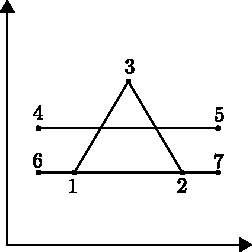
\includegraphics{./img/ch2-edgeint.pdf}
    \caption{The bunch of edges used for the tests.}
\end{figure}
@D planar\_arrangement support functions tests
@{@@testset "Edge fragmentation tests" begin
    V = [2 2; 4 2; 3 3.5; 1 3; 5 3; 1 2; 5 2]
    EV = sparse(Array{Int8, 2}([
        [1 1 0 0 0 0 0] #1->12
        [0 1 1 0 0 0 0] #2->23
        [1 0 1 0 0 0 0] #3->13
        [0 0 0 1 1 0 0] #4->45
        [0 0 0 0 0 1 1] #5->67
    ]))

    @@testset "intersect_edges" begin
        inters1 = LARLIB.intersect_edges(V, EV[5, :], EV[1, :])
        inters2 = LARLIB.intersect_edges(V, EV[1, :], EV[4, :])
        inters3 = LARLIB.intersect_edges(V, EV[1, :], EV[2, :])
        @@test inters1 == [([2. 2.], 1/4),([4. 2.], 3/4)]
        @@test inters2 == []
        @@test inters3 == [([4. 2.], 1)]
    end

    @@testset "frag_edge" begin
        rV, rEV = LARLIB.frag_edge(V, EV, 5)
        @@test rV == [2.0 2.0; 4.0 2.0; 3.0 3.5; 1.0 3.0; 
                     5.0 3.0; 1.0 2.0; 5.0 2.0; 2.0 2.0; 
                     4.0 2.0; 4.0 2.0; 2.0 2.0]
        @@test full(rEV) == [0 0 0 0 0 1 0 0 0 0 1; 
                            0 0 0 0 0 0 0 0 0 1 1;
                            0 0 0 0 0 0 1 0 0 1 0]
    end
end
@}









%%%%%%%%%%%%%%%%%%%%%%%%%%%%%%%%%%%
\section{Coincident vertices merge}
\label{sec:2D_merge_vertices}

To merge vertices in $d=2$ the procedure is obviously similar to the one 
used for $d=3$ so we will
reuse some macros already defined [ref. \ref{sec:3D_merge_vertices}]

@D LAR imports
@{using NearestNeighbors
@}

The function is marked with ``\texttt{!}'' in its signature 
because it has collateral effects
on the \texttt{edge\_map} argument; we will for sure modify both
the geometry and the topology of the complex, so \texttt{edge\_map}
must be accordingly updated.

@D planar\_arrangement support functions
@{function merge_vertices!(V::Verts, EV::Cells, edge_map, err=1e-4)
    vertsnum = size(V, 1)
    edgenum = size(EV, 1)
    newverts = zeros(Int, vertsnum)
    kdtree = KDTree(V')

    @< Find coincident vertices @>
    @< Merge edges @>
    @< Update edge\_map after vertex merging @>

    return nV, nEV
end
@}

The last step is to update \texttt{edge\_map}.
We update the indices using the data structures
built in the $\langle$ Merge edges $\rangle$ macro
[ref. \ref{sec:3D_merge_vertices}].

@D Update edge\_map after vertex merging
@{for i in 1:length(edge_map)
    row = edge_map[i]
    row = map(x->edges[x], row)
    row = filter(t->t[1]!=t[2], row)
    row = map(x->etuple2idx[x], row)
    edge_map[i] = row
end
@}


%+++++++++++++++++++++++++%
\subsection{Implementation}
We simply call \texttt{merge\_vertices}.
@D Merge coincident vertices
@{V, EV = merge_vertices!(V, EV, edge_map)
@}
%++++++++++++++++%
\subsection{Tests}
Let's merge the vertices of a square built by numerous
very similar edges.
@D planar\_arrangement support functions tests
@{@@testset "merge_vertices test set" begin
    n0 = 1e-12
    n1l = 1-1e-12
    n1u = 1+1e-12
    V = [ n0  n0; -n0  n0;  n0 -n0; -n0 -n0;
          n0 n1u; -n0 n1u;  n0 n1l; -n0 n1l;
         n1u n1u; n1l n1u; n1u n1l; n1l n1l;
         n1u  n0; n1l  n0; n1u -n0; n1l -n0]
    EV = Int8[1 0 0 0 1 0 0 0 0 0 0 0 0 0 0 0;
              0 1 0 0 0 1 0 0 0 0 0 0 0 0 0 0;
              0 0 1 0 0 0 1 0 0 0 0 0 0 0 0 0;
              0 0 0 1 0 0 0 1 0 0 0 0 0 0 0 0;
              0 0 0 0 1 0 0 0 1 0 0 0 0 0 0 0;
              0 0 0 0 0 1 0 0 0 1 0 0 0 0 0 0;
              0 0 0 0 0 0 1 0 0 0 1 0 0 0 0 0;
              0 0 0 0 0 0 0 1 0 0 0 1 0 0 0 0;
              0 0 0 0 0 0 0 0 1 0 0 0 1 0 0 0;
              0 0 0 0 0 0 0 0 0 1 0 0 0 1 0 0;
              0 0 0 0 0 0 0 0 0 0 1 0 0 0 1 0;
              0 0 0 0 0 0 0 0 0 0 0 1 0 0 0 1;
              1 0 0 0 0 0 0 0 0 0 0 0 1 0 0 0;
              0 1 0 0 0 0 0 0 0 0 0 0 0 1 0 0;
              0 0 1 0 0 0 0 0 0 0 0 0 0 0 1 0;
              0 0 0 1 0 0 0 0 0 0 0 0 0 0 0 1]
    EV = sparse(EV)
    V, EV = LARLIB.merge_vertices!(V, EV, [])

    @@test V == [n0 n0; n0 n1u; n1u n1u; n1u n0]
    @@test full(EV) == [1 1 0 0;
                       0 1 1 0;
                       0 0 1 1;
                       1 0 0 1]
end
@}



%%%%%%%%%%%%%%%%%%%%%%%%%%%%%%%%%%%%%%%%%%%%
\section{Delete edges outside $\sigma$ area}

If a face $\sigma$ is passed as input of the planar arrangement,
we need to delete the edges outside the area of $\sigma$. 
First, we use \texttt{edge\_map} to get the fragments of the edges of the original $\sigma$;
then for every edge which is not a fragment of $\sigma$'s edges, we check if its centroid
is inside $\sigma$ using the \texttt{point\_in\_face} utility [ref. \ref{sec:point_in_face}].
Finally, once we have marked the edges to delete, we delete them [ref. \ref{sec:delete_edges}] 
and update the \texttt{edge\_map} (refer to next macro for this).

@D Delete edges outside sigma area
@{if sigma.n > 0
    todel = []
    
    new_edges = []
    map(i->new_edges=union(new_edges, edge_map[i]), sigma.nzind)
    ev = EV[new_edges, :]

    for e in 1:EV.m
        if !(e in new_edges)

            vidxs = EV[e, :].nzind
            v1, v2 = map(i->V[vidxs[i], :], [1,2])
            centroid = .5*(v1 + v2)
            
            if !point_in_face(centroid, V, ev) 
                push!(todel, e)
            end
        end
    end

    @< Update edge\_map @>

    V, EV = delete_edges(todel, V, EV)
end
@}

\label{macro:update_edge_map}
For every deleted edge the \texttt{edge\_map} must be updated. 
So we delete the index of the edge from the mapping and subtract one 
to the indices greater than the index of the deleted edge.


@D Update edge\_map
@{for i in reverse(todel)
    for row in edge_map

        filter!(x->x!=i, row)

        for j in 1:length(row)
            if row[j] > i
                row[j] -= 1
            end
        end
    end
end
@}




%%%%%%%%%%%%%%%%%%%%%%%%%%%%%%%%%%%%%%%%
\section{Maximal biconnected components}
\begin{figure}[h]
    \centering
    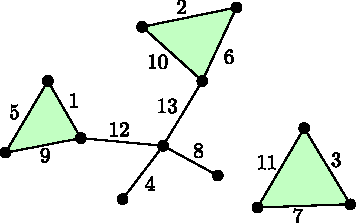
\includegraphics{./img/ch2-bicon.pdf}
    \caption{An example graph where the maximal biconnected 
    components are highlighted in green and the edges are numbered. 
    We have here three components formed by the sets of edges \{1,5,9\}, \{2,6,10\} and \{3,11,7\} }
    \label{img:bicon_comps}
\end{figure}
%+++++++++++++++++++++++++++%
\subsection{Support function}
\label{sec:biconnected_components}
To individuate the maximal biconnected components of the fragmented and merged 1-skeleton
we use the 1973 Hopcroft-Tarjan algorithm for biconnected components\cite{Hopcroft-Tarjan}.
@D planar\_arrangement support functions
@{function biconnected_components(EV::Cells)
    @< biconnected\_components local variables @>
    @< DFS utilities @>
    @< Depth first visit @>
    bicon_comps
end
@}
We will need a point stack (\texttt{ps}), an edge stack (\texttt{es}), a list of traversed edges (\texttt{todel}), a list of 
visited points (\texttt{visited}), a list of biconnected components (\texttt{bicon\_comps}) and a index to avoid duplicate 
numbering of vertices (\texttt{hivtx}). \texttt{ps} is made of triples composed by the index of the vertex in \texttt{V}, 
the index assigned by the algorithm and the component identifier also assigned by the algorithm. \texttt{es} instead 
contains couples with the index of the edge inside \texttt{EV} and the assigned index of the tail node. The indexes 
in \texttt{todel} and \texttt{bicon\_comps} are relative to \texttt{EV} while the ones of \texttt{visited} are
relative to \texttt{V}
@D biconnected\_components local variables
@{ps = Array{Tuple{Int, Int, Int}, 1}()
es = Array{Tuple{Int, Int}, 1}()
todel = Array{Int, 1}()
visited = Array{Int, 1}()
bicon_comps = Array{Array{Int, 1}, 1}()
hivtx = 1
@}
Here are implemented some functions helpful throughout the algorithm.
\texttt{an\_edge} returns the index relative to \texttt{EV} of the first edge out of \texttt{point} if exists or 
\texttt{false} otherwise. \texttt{get\_head}, given an \texttt{edge} and a point (the \texttt{tail}), returns the 
index relative to \texttt{V} of the head (the point that is not \texttt{tail}) of the \texttt{edge}. 
\texttt{v\_to\_vi}, given the index relative to \texttt{V} of a vertex (\texttt{v}), returns its index using 
the algorithm numbering. This index can also not exists; in this case \texttt{false} is returned.
@D DFS utilities
@{function an_edge(point)
    edges = setdiff(EV[:, point].nzind, todel)
    if length(edges) == 0
        edges = [false]
    end
    edges[1]
end

function get_head(edge, tail)
    setdiff(EV[edge, :].nzind, [tail])[1]
end

function v_to_vi(v)
    i = findfirst(t->t[1]==v, ps)
    if i == 0
        return false
    else
        return ps[i][2]
    end
end
@}
The DFS visit is mostly akin to the one proposed in the Hopcroft-Tarjan original algorithm.
The starting point is the first one in \texttt{V}.
@D Depth first visit
@{push!(ps, (1,1,1))
push!(visited, 1)
exit = false
while !exit
    edge = an_edge(ps[end][1])
    if edge != false
        tail = ps[end][2]
        head = get_head(edge, ps[end][1])
        hi = v_to_vi(head)
        if hi == false
            hivtx += 1
            push!(ps, (head, hivtx, ps[end][2]))
            push!(visited, head)
        else
            if hi < ps[end][3]
                ps[end] = (ps[end][1], ps[end][2], hi)
            end
        end
        push!(es, (edge, tail))
        push!(todel, edge)
    else
        if length(ps) == 1
            @< Handle disconnected graph @>
        else
            if ps[end][3] == ps[end-1][2]
                @< Form biconnected component @>
            else
                if ps[end-1][3] > ps[end][3]
                    ps[end-1] = (ps[end-1][1], ps[end-1][2], ps[end][3])
                end
            end
            pop!(ps)
        end
    end
end
@}
To form a biconnected component we pop edges out from the stack of edges (\texttt{es}) until we find the one
of which the index of its tail is equal to the component identifier (called \texttt{LOWPOINT} in the original algorithm) 
of the top point of the point stack (\texttt{ps}). We effectively put inside the \texttt{bicon\_comps} only the components
made of more than one edge because we are interested in building a 1-skeleton of valid 2-cells.
@D Form biconnected component
@{edges = Array{Int, 1}()
while true
    edge, tail = pop!(es)
    push!(edges, edge)
    if tail == ps[end][3]
        if length(edges) > 1
            push!(bicon_comps, edges)
        end
        break
    end
end
@}
When there are no more points to visit in the current connected component we search for a point in \texttt{V}
which has not been visited yet (so a point not listed in the \texttt{visited} array) and we put it on the top
of a new point stack and then let the algorithm iterate again. If there are no more new connected components 
to visit we break the algorithm iteration and exit.
@D Handle disconnected graph
@{found = false
pop!(ps)
for i in 1:size(EV,2)
    if !(i in visited)
        hivtx = 1
        push!(ps, (i, hivtx, 1))
        push!(visited, i)
        found = true
        break
    end
end
if !found
    exit = true
end
@}
%+++++++++++++++++++++++++%
\subsection{Implementation}
Like for the vertices merge we simply call the freshly implemented \texttt{biconnected\_components} function
[ref. \ref{sec:biconnected_components}]. If no biconnected components are found, the procedure will stop and return nothing.
@D Find maximal biconnected components
@{bicon_comps = biconnected_components(EV)

if isempty(bicon_comps)
    println("No biconnected components found.")
    return (nothing, nothing, nothing)
end
@}

We also need to delete edges that are not part of a maximal biconnected component
and then to delete the isolated vertices from both \texttt{V} and \texttt{EV}.
We also update the \texttt{edge\_map} to adapt it to the deletions made (We use the
macro defined in \ref{macro:update_edge_map}).

@D Filter biconnected components
@{
edges = sort(union(bicon_comps...))
todel = sort(setdiff(collect(1:size(EV,1)), edges))

@< Update edge\_map @>

V, EV = delete_edges(todel, V, EV)

@}

%++++++++++++++++%
\subsection{Tests}
The graph built here is the one of figure \ref{img:bicon_comps}.
@D planar\_arrangement support functions tests
@{@@testset "biconnected_components test set" begin
    EV = Int8[0 0 0 1 0 0 0 0 0 0 1 0; #1
              0 0 1 0 0 1 0 0 0 0 0 0; #2
              0 0 0 0 0 0 1 0 0 1 0 0; #3
              1 0 0 0 1 0 0 0 0 0 0 0; #4
              0 0 0 1 0 0 0 1 0 0 0 0; #5
              0 0 1 0 0 0 0 0 1 0 0 0; #6
              0 1 0 0 0 0 0 0 0 1 0 0; #7
              0 0 0 0 1 0 0 0 0 0 0 1; #8
              0 0 0 0 0 0 0 1 0 0 1 0; #9
              0 0 0 0 0 1 0 0 1 0 0 0; #10
              0 1 0 0 0 0 1 0 0 0 0 0; #11
              0 0 0 0 1 0 0 0 0 0 1 0; #12
              0 0 0 0 1 0 0 0 1 0 0 0] #13
    EV = sparse(EV)

    bc = LARLIB.biconnected_components(EV)
    bc = Set(map(Set, bc))

    @@test bc == Set([Set([1,5,9]), Set([2,6,10]), Set([3,7,11])])
end
@}













%%%%%%%%%%%%%%%%%%%%%%%%
\section{Faces creation}
%+++++++++++++++++++++++++%
\subsection{Implementation}
@D Create faces
@{bicon_comps = biconnected_components(EV)

n = size(bicon_comps, 1)
shells = Array{Cell, 1}(n)
boundaries = Array{Cells, 1}(n)
EVs = Array{Cells, 1}(n)
for p in 1:n
    ev = EV[sort(bicon_comps[p]), :]
    fe = minimal_2cycles(V, ev)
    shell_num = get_external_cycle(V, ev, fe)

    EVs[p] = ev 
    tokeep = setdiff(1:fe.m, shell_num)
    boundaries[p] = fe[tokeep, :]
    shells[p] = fe[shell_num, :]
end

@< Containment test @>
@< Transitive reduction @>
@< Cell merging @>

@}

%++++++++++++++++++++++++++++++++++++++++%
\subsection{Individuate the external cell}
Once we computed the minimal 2-cycles [ref. \ref{ch:minimal_cycles}]
we need to individuate the external cycle. To do this we iterate over the
vertices of the passed \texttt{EV} to find four vertices: the two with biggest
$x_1$ and $x_2$ coordinates (\texttt{maxv\_x1} and \texttt{maxv\_x2}) and the 
two with the smallest one (\texttt{minv\_x1} and \texttt{minv\_x2}). 
Then we check which face the two vertices have in common. 

It can happen that the two vertices have more than one face in common
(for example when a biconnected component is made up only by one face);
in this case we simply pick the cell with negative area. The area
computation routines are located into section \ref{sec:face_area},


@D planar\_arrangement support functions
@{function get_external_cycle(V::Verts, EV::Cells, FE::Cells)
    FV = abs.(FE)*EV
    vs = sparsevec(mapslices(sum, abs.(EV), 1)).nzind
    minv_x1 = maxv_x1 = minv_x2 = maxv_x2 = pop!(vs)
    for i in vs
        if V[i, 1] > V[maxv_x1, 1]
            maxv_x1 = i
        elseif V[i, 1] < V[minv_x1, 1]
            minv_x1 = i
        end
        if V[i, 2] > V[maxv_x2, 2]
            maxv_x2 = i
        elseif V[i, 2] < V[minv_x2, 2]
            minv_x2 = i
        end
    end
    cells = intersect(
        FV[:, minv_x1].nzind, 
        FV[:, maxv_x1].nzind,
        FV[:, minv_x2].nzind,
        FV[:, maxv_x2].nzind
    )
    if length(cells) == 1
        return cells[1]
    else
        for c in cells
            if face_area(V, EV, FE[c, :]) < 0
                return c
            end
        end
    end
end
@}

%+++++++++++++++++++++++++++%
\subsection{Containment test}

For each shell we must compute if it is contained
in another shell. So, for every couple of shells
we must check if one is contained into the other.
This check must be performed by shooting a ray from
a vertex of the first cell and then count the intersections
of it with the edges of the second cell; if the number 
of the intersections is odd then the first cell is contained
in the second one. This computation is rather heavy but can be
speeded up by pre-computing an approximate containment graph 
using a bounding box containment test. Then the graph must be
pruned shooting a ray for every arc of it. In this way we reduce
considerably the amount of rays we shoot. This will be also visually
explained in the tests [ref. \ref{sec:conttest_test}].

Before building the containment graph, we
compute the bounding boxes of the shells and we store them into
the \texttt{shell\_bboxes} list (we are going to use this also later).
The bounding box logic is implemented in the utilities
[ref. \ref{sec:bboxes}].

@D Containment test
@{shell_bboxes = []
for i in 1:n
    vs_indexes = (abs.(EVs[i]')*abs.(shells[i])).nzind
    push!(shell_bboxes, bbox(V[vs_indexes, :]))
end

containment_graph = pre_containment_test(shell_bboxes)
containment_graph = prune_containment_graph(n, V, EVs, shells, containment_graph)
@}

@D planar\_arrangement support functions
@{function pre_containment_test(bboxes)
    n = length(bboxes)
    containment_graph = spzeros(Int8, n, n)

    for i in 1:n
        for j in 1:n
            if i != j && bbox_contains(bboxes[j], bboxes[i])
                containment_graph[i, j] = 1
            end
        end
    end

    return containment_graph
end
@}

To check if a point is really inside a face we use the
\texttt{point\_in\_face} utility [ref. \ref{sec:point_in_face}]

@D planar\_arrangement support functions
@{function prune_containment_graph(n, V, EVs, shells, graph)
    
    for i in 1:n
        an_edge = shells[i].nzind[1]
        origin_index = EVs[i][an_edge, :].nzind[1]
        origin = V[origin_index, :]
 
        for j in 1:n
            if i != j
                if graph[i, j] == 1
                    shell_edge_indexes = shells[j].nzind
                    ev = EVs[j][shell_edge_indexes, :]

                    if !point_in_face(origin, V, ev)
                        graph[i, j] = 0
                    end
                end
             end
         end

     end
     return graph
end
@}

%+++++++++++++++++++++++++++++++%
\subsection{Transitive reduction}

We have an adjacency matrix and we must perform a transitive reduction.
As explained by A. V. Aho, M. R. Garey, and J. D. Ullman \cite{transitive_reduction}
we have:

@D Transitive reduction
@{transitive_reduction!(containment_graph) 
@}

@D planar\_arrangement support functions
@{function transitive_reduction!(graph)
    n = size(graph, 1)
    for j in 1:n
        for i in 1:n
            if graph[i, j] > 0
                for k in 1:n
                    if graph[j, k] > 0
                        graph[i, k] = 0
                    end
                end
            end
        end
    end
end
@}

%+++++++++++++++++++++++%
\subsection{Cell merging}

For every arc of the containment tree we have a father component 
and a child component and we must find the cycle of the father that
contains the child. This happens if the bounding box of the child is fully
contained in the box of the cycle\footnote{Please note that
that the \texttt{bboxes} is not part of the bounding box utilities 
[ref. \ref{sec:bboxes}] but it is defined 
in the next paragraph}. The \texttt{sums} array contains the indexes of 
the rows of the various boundary matrices to sum after the containment 
graph has been traversed. Every element is a triple made of: the father 
index, the father's container cell index and the child index.
Once we individuated the rows to sum, we actually need to perform the sum.
This is non trivial because we must build the final boundary matrix.
These computations are delegated to the $\langle$ Create EV and FE $\rangle$ macro.
@D Cell merging 
@{EV, FE = cell_merging(n, containment_graph, V, EVs, boundaries, shells, shell_bboxes)
@}

@D planar\_arrangement support functions 
@{function cell_merging(n, containment_graph, V, EVs, boundaries, shells, shell_bboxes)
    @< Cell merging support functions @>

    sums = Array{Tuple{Int, Int, Int}}(0);

    for father in 1:n
        if sum(containment_graph[:, father]) > 0
            father_bboxes = bboxes(V, abs.(EVs[father]')*abs.(boundaries[father]'))
            for child in 1:n
                if containment_graph[child, father] > 0
                    child_bbox = shell_bboxes[child]
                    for b in 1:length(father_bboxes)
                        if bbox_contains(father_bboxes[b], child_bbox)
                            push!(sums, (father, b, child))
                            break
                        end
                    end
                end            
            end
        end
    end

    @< Create EV and FE @>
    return EV, FE
end
@}

The \texttt{bboxes} computes the bounding boxes of each cycle
described in the \texttt{indexes} matrix.

@D Cell merging support functions
@{function bboxes(V::Verts, indexes::Cells)
    boxes = Array{Tuple{Any, Any}}(indexes.n)
    for i in 1:indexes.n
        v_inds = indexes[:, i].nzind
        boxes[i] = bbox(V[v_inds, :])
    end
    boxes
end
@}

To actually build the complete and correct boundary matrix \texttt{FE},
we compute the final dimensions of it, then we initialize it filled with
zeros and then we fill it with the correct data in the correct position.
While doing this we store into \texttt{c\_offsets} the column offset of each
biconnected component; we will use this information to quickly find the columns 
to sum from the \texttt{sums} array of triples.

@D Create EV and FE
@{EV = vcat(EVs...)
edgenum = size(EV, 1)
facenum = sum(map(x->size(x,1), boundaries))
FE = spzeros(Int8, facenum, edgenum)
shells2 = spzeros(Int8, length(shells), edgenum)
r_offsets = [1]
c_offset = 1
for i in 1:n
    min_row = r_offsets[end]
    max_row = r_offsets[end] + size(boundaries[i], 1) - 1
    min_col = c_offset
    max_col = c_offset + size(boundaries[i], 2) - 1
    FE[min_row:max_row, min_col:max_col] = boundaries[i]
    shells2[i, min_col:max_col] = shells[i]
    push!(r_offsets, max_row + 1)
    c_offset = max_col + 1
end

for (f, r, c) in sums
    FE[r_offsets[f]+r-1, :] += shells2[c, :]
end
@}


%++++++++++++++++%
\subsection{Tests}

@D planar\_arrangement support functions tests
@{@@testset "Face creation" begin
    @< Face creation tests @>
end
@}

\subsubsection{External cell individuation}
\begin{figure}[h]
    \centering
    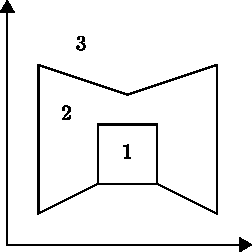
\includegraphics{./img/ch2-externcell.pdf}
    \caption{This biconnected component has three faces. The external one is the number 3.
    This is a particularly difficult case because the most "external" vertices of face 2
    are in common with the external cell.}
\end{figure}

@D Face creation tests
@{@@testset "External cell individuation" begin
    V = [ .5 .5;  1.5   1;  1.5  2; 
         2.5  2;  2.5   1;  3.5 .5;
         3.5  3;    2 2.5;   .5  3]

    EV = Int8[-1  1  0  0  0  0  0  0  0;
               0 -1  1  0  0  0  0  0  0;
               0  0 -1  1  0  0  0  0  0;
               0  0  0 -1  1  0  0  0  0;
               0  0  0  0 -1  1  0  0  0;
               0  0  0  0  0 -1  1  0  0;
               0  0  0  0  0  0 -1  1  0;
               0  0  0  0  0  0  0 -1  1;
              -1  0  0  0  0  0  0  0  1;
               0 -1  0  0  1  0  0  0  0]
    EV = sparse(EV)
    
    FE = Int8[ 0 -1 -1 -1  0  0  0  0  0  1;
               1  1  1  1  1  1  1  1 -1  0;
              -1  0  0  0 -1 -1 -1 -1  1 -1]
    FE = sparse(FE)

    @@test LARLIB.get_external_cycle(V, EV, FE) == 3
end
@}

\subsubsection{Containment test}
\label{sec:conttest_test}

\begin{figure}[h]
    \centering
    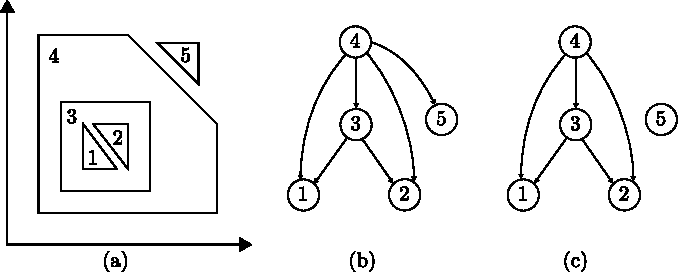
\includegraphics{./img/ch2-containmenttest.pdf}
    \caption{(a) is our test case. The numbers identify the connected components. 
        (b) is the containment graph built using only the \texttt{pre\_containment\_test} 
        function. The arc (4,5) is in there because the bounding box of the component 
        no. 5 is completely contained in the bounding box of no. 4. (c) shows 
        the graph after the \texttt{prune\_containment\_graph} function.}
\end{figure}

@D Face creation tests
@{@@testset "Containment test" begin
    V = [  0   0;    4   0;    4   2;   2   4;  0 4;
          .5  .5;  2.5  .5;  2.5 2.5;  .5 2.5;
           1   1;  1.5   1;    1   2;
           2   1;    2   2;  1.5   2;
         3.5 3.5;    3 3.5;  3.5   3]
    EV1 = Int8[ 0  0  0  0  0  0  0  0  0 -1  1  0  0  0  0  0  0  0;
                0  0  0  0  0  0  0  0  0  0 -1  1  0  0  0  0  0  0;
                0  0  0  0  0  0  0  0  0 -1  0  1  0  0  0  0  0  0]
    EV2 = Int8[ 0  0  0  0  0  0  0  0  0  0  0  0 -1  1  0  0  0  0;
                0  0  0  0  0  0  0  0  0  0  0  0  0 -1  1  0  0  0;
                0  0  0  0  0  0  0  0  0  0  0  0 -1  0  1  0  0  0]
    EV3 = Int8[ 0  0  0  0  0 -1  1  0  0  0  0  0  0  0  0  0  0  0;
                0  0  0  0  0  0 -1  1  0  0  0  0  0  0  0  0  0  0;
                0  0  0  0  0  0  0 -1  1  0  0  0  0  0  0  0  0  0;
                0  0  0  0  0 -1  0  0  1  0  0  0  0  0  0  0  0  0]
    EV4 = Int8[-1  1  0  0  0  0  0  0  0  0  0  0  0  0  0  0  0  0;
                0 -1  1  0  0  0  0  0  0  0  0  0  0  0  0  0  0  0;
                0  0 -1  1  0  0  0  0  0  0  0  0  0  0  0  0  0  0;
                0  0  0 -1  1  0  0  0  0  0  0  0  0  0  0  0  0  0;
               -1  0  0  0  1  0  0  0  0  0  0  0  0  0  0  0  0  0]
    EV5 = Int8[ 0  0  0  0  0  0  0  0  0  0  0  0  0  0  0 -1  1  0;
                0  0  0  0  0  0  0  0  0  0  0  0  0  0  0  0 -1  1;
                0  0  0  0  0  0  0  0  0  0  0  0  0  0  0 -1  0  1]
    EVs = map(sparse, [EV1, EV2, EV3, EV4, EV5])
    
    shell1 = Int8[-1 -1  1];
    shell2 = Int8[-1 -1  1];
    shell3 = Int8[-1 -1 -1  1];
    shell4 = Int8[-1 -1 -1 -1  1];
    shell5 = Int8[-1 -1  1];
    shells = map(sparsevec, [shell1, shell2, shell3, shell4, shell5])
    
    shell_bboxes = []
    n = 5
    for i in 1:n
        vs_indexes = (abs.(EVs[i]')*abs.(shells[i])).nzind
        push!(shell_bboxes, LARLIB.bbox(V[vs_indexes, :]))
    end

    graph = LARLIB.pre_containment_test(shell_bboxes)
    @@test graph == [0 0 1 1 0; 0 0 1 1 0; 0 0 0 1 0; 0 0 0 0 0; 0 0 0 1 0]

    graph = LARLIB.prune_containment_graph(n, V, EVs, shells, graph)
    @@test graph == [0 0 1 1 0; 0 0 1 1 0; 0 0 0 1 0; 0 0 0 0 0; 0 0 0 0 0]
end
@}

\subsubsection{Transitive reduction}
\label{sec:transitivered_test}

\begin{figure}[h]
    \centering
    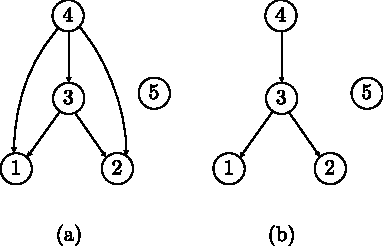
\includegraphics{./img/ch2-transitivered.pdf}
    \caption{Before (a) and after (b) transitive reduction performed on
    the graph of the previous test set.}
\end{figure}

@D Face creation tests
@{@@testset "Transitive reduction" begin
    graph = [0 0 1 1 0; 0 0 1 1 0; 0 0 0 1 0; 0 0 0 0 0; 0 0 0 0 0]
    LARLIB.transitive_reduction!(graph)
    @@test graph == [0 0 1 0 0; 0 0 1 0 0; 0 0 0 1 0; 0 0 0 0 0; 0 0 0 0 0]
end
@}

\subsubsection{Cell merging}

\begin{figure}[h]
    \centering
    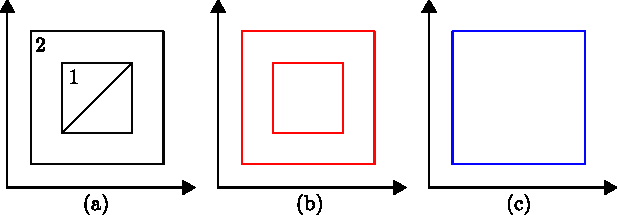
\includegraphics{./img/ch2-cellmerge.pdf}
    \caption{Here we have two biconnected components, one inside the other (a).
    If we don't perform cell merging, the boundary of the arranged set will be
    the red one (b), which is incorrect. The correct boundary is the blue one (c).}
\end{figure}

@D Face creation tests
@{@@testset "Cell merging" begin
    graph = [0 1; 0 0]
    V = [.25 .25; .75 .25; .75 .75; .25 .75;
           0   0;   1   0;   1   1;   0   1]
    EV1 = Int8[-1  1  0  0  0  0  0  0;
                0 -1  1  0  0  0  0  0;
                0  0 -1  1  0  0  0  0;
               -1  0  0  1  0  0  0  0;
               -1  0  1  0  0  0  0  0]
    EV2 = Int8[ 0  0  0  0 -1  1  0  0;
                0  0  0  0  0 -1  1  0;
                0  0  0  0  0  0 -1  1;
                0  0  0  0 -1  0  0  1]
    EVs = map(sparse, [EV1, EV2])

    shell1 = Int8[-1 -1 -1  1  0]
    shell2 = Int8[-1 -1 -1  1]
    shells = map(sparsevec, [shell1, shell2])

    boundary1 = Int8[ 1  1  0  0 -1;
                      0  0  1 -1  1]
    boundary2 = Int8[ 1  1  1 -1]
    boundaries = map(sparse, [boundary1, boundary2])

    shell_bboxes = []
    n = 2
    for i in 1:n
        vs_indexes = (abs.(EVs[i]')*abs.(shells[i])).nzind
        push!(shell_bboxes, LARLIB.bbox(V[vs_indexes, :]))
    end

    EV, FE = LARLIB.cell_merging(2, graph, V, EVs, boundaries, shells, shell_bboxes)

    selector = sparse(ones(Int8, 1, 3))

    @@test selector*FE == [0  0  0  0  0  1  1  1 -1]
end
@}


%%%%%%%%%%%%%%%%%%%%%%%%
\section{General examples}
\label{sec:planar_arrangement_examples}

@D planar\_arrangement general examples
@{function generate_perpendicular_lines(steps::Int, minlen, maxlen)
    V = zeros(0,2)

    function rec(o, d, s)
        if s == 0 return end

        a = (maxlen-minlen)*rand() + minlen
        p = o + a*d
        V = [V; o; p]

        b = (a-minlen)*rand() + minlen
        p = o + b*d
        rec(p, d, s-1)

        b = (a-minlen)*rand() + minlen
        p = o + b*d
        rec(p, perpendicular(d), s-1)
    end

    function perpendicular(vec)
        v = zeros(size(vec))
        v[1] = vec[2]
        v[2] = vec[1]
        return v
    end

    rec([0 0], [1 0], steps)
    rec([0 0], [0 1], steps)
    vnum = size(V, 1)
    enum = vnum >> 1
    EV = spzeros(Int8, enum, vnum)
    for i in 1:enum
        EV[i, i*2-1:i*2] = 1
    end
    V, EV
end


function generate_random_lines(n, points_range, alphas_range)
    origins = points_range[1] + (points_range[2]-points_range[1])*rand(n, 2)
    directions = mapslices(normalize, rand(n, 2) - .5*ones(n, 2), 2)
    alphas = alphas_range[1] + (alphas_range[2]-alphas_range[1])*rand(n)
    new_points = Array{Float64, 2}(n, 2)
    for i in 1:n
        new_points[i, :] = origins[i, :] + alphas[i]*directions[i, :]
    end
    V = [origins; new_points]
    EV = spzeros(Int8, n, n*2)
    for i in 1:n
        EV[i, i] = 1
        EV[i, n+i] = 1
    end
    V, EV
end
@}

\vfill

\begin{figure}[p!]
    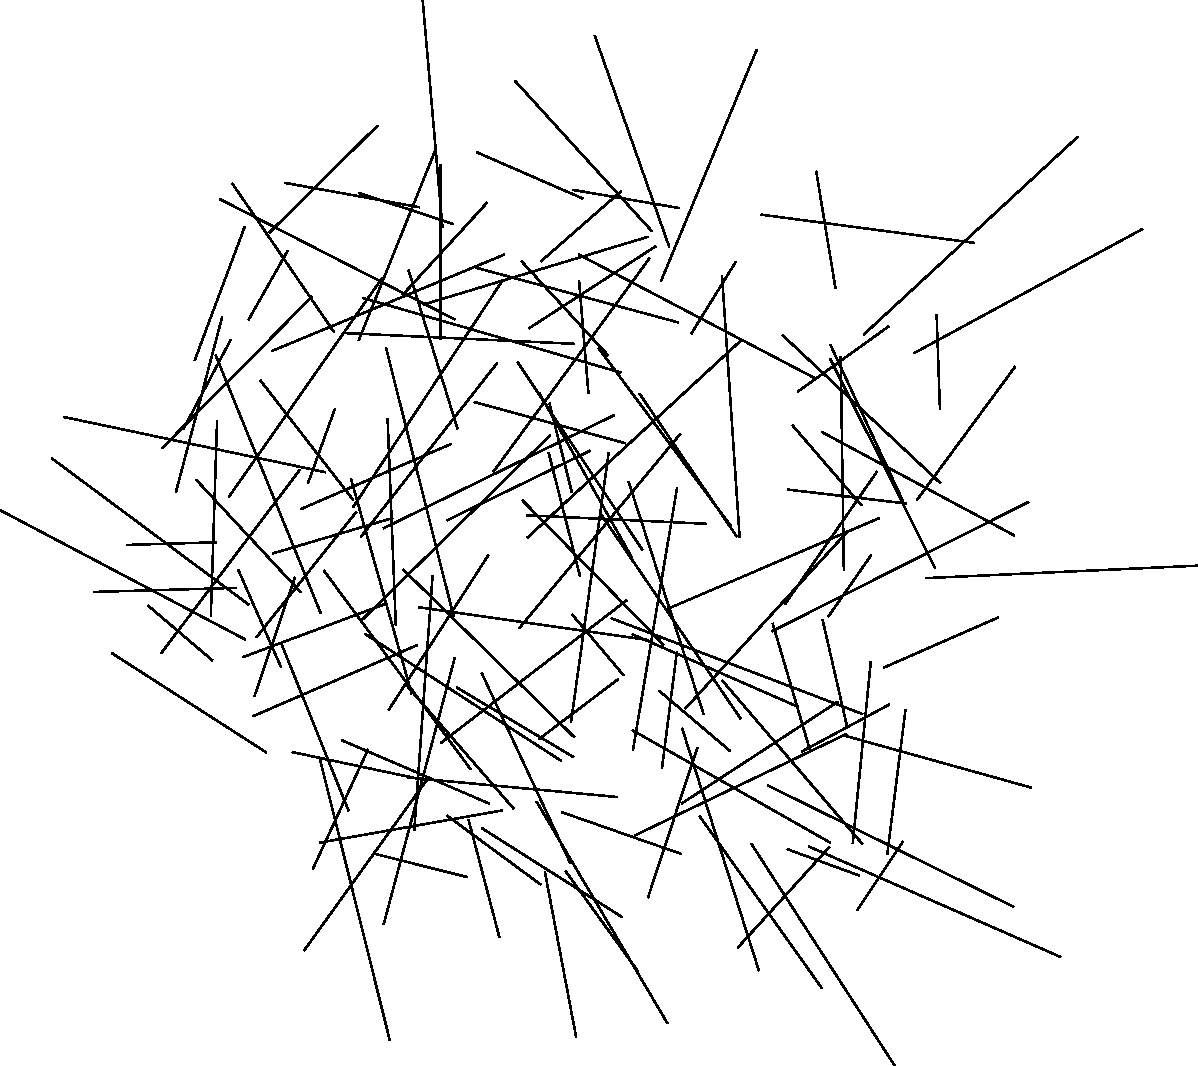
\includegraphics[width=\textwidth]{./img/test-lines.pdf}%
    \caption{Input}
\end{figure}


\begin{figure}[p!]
    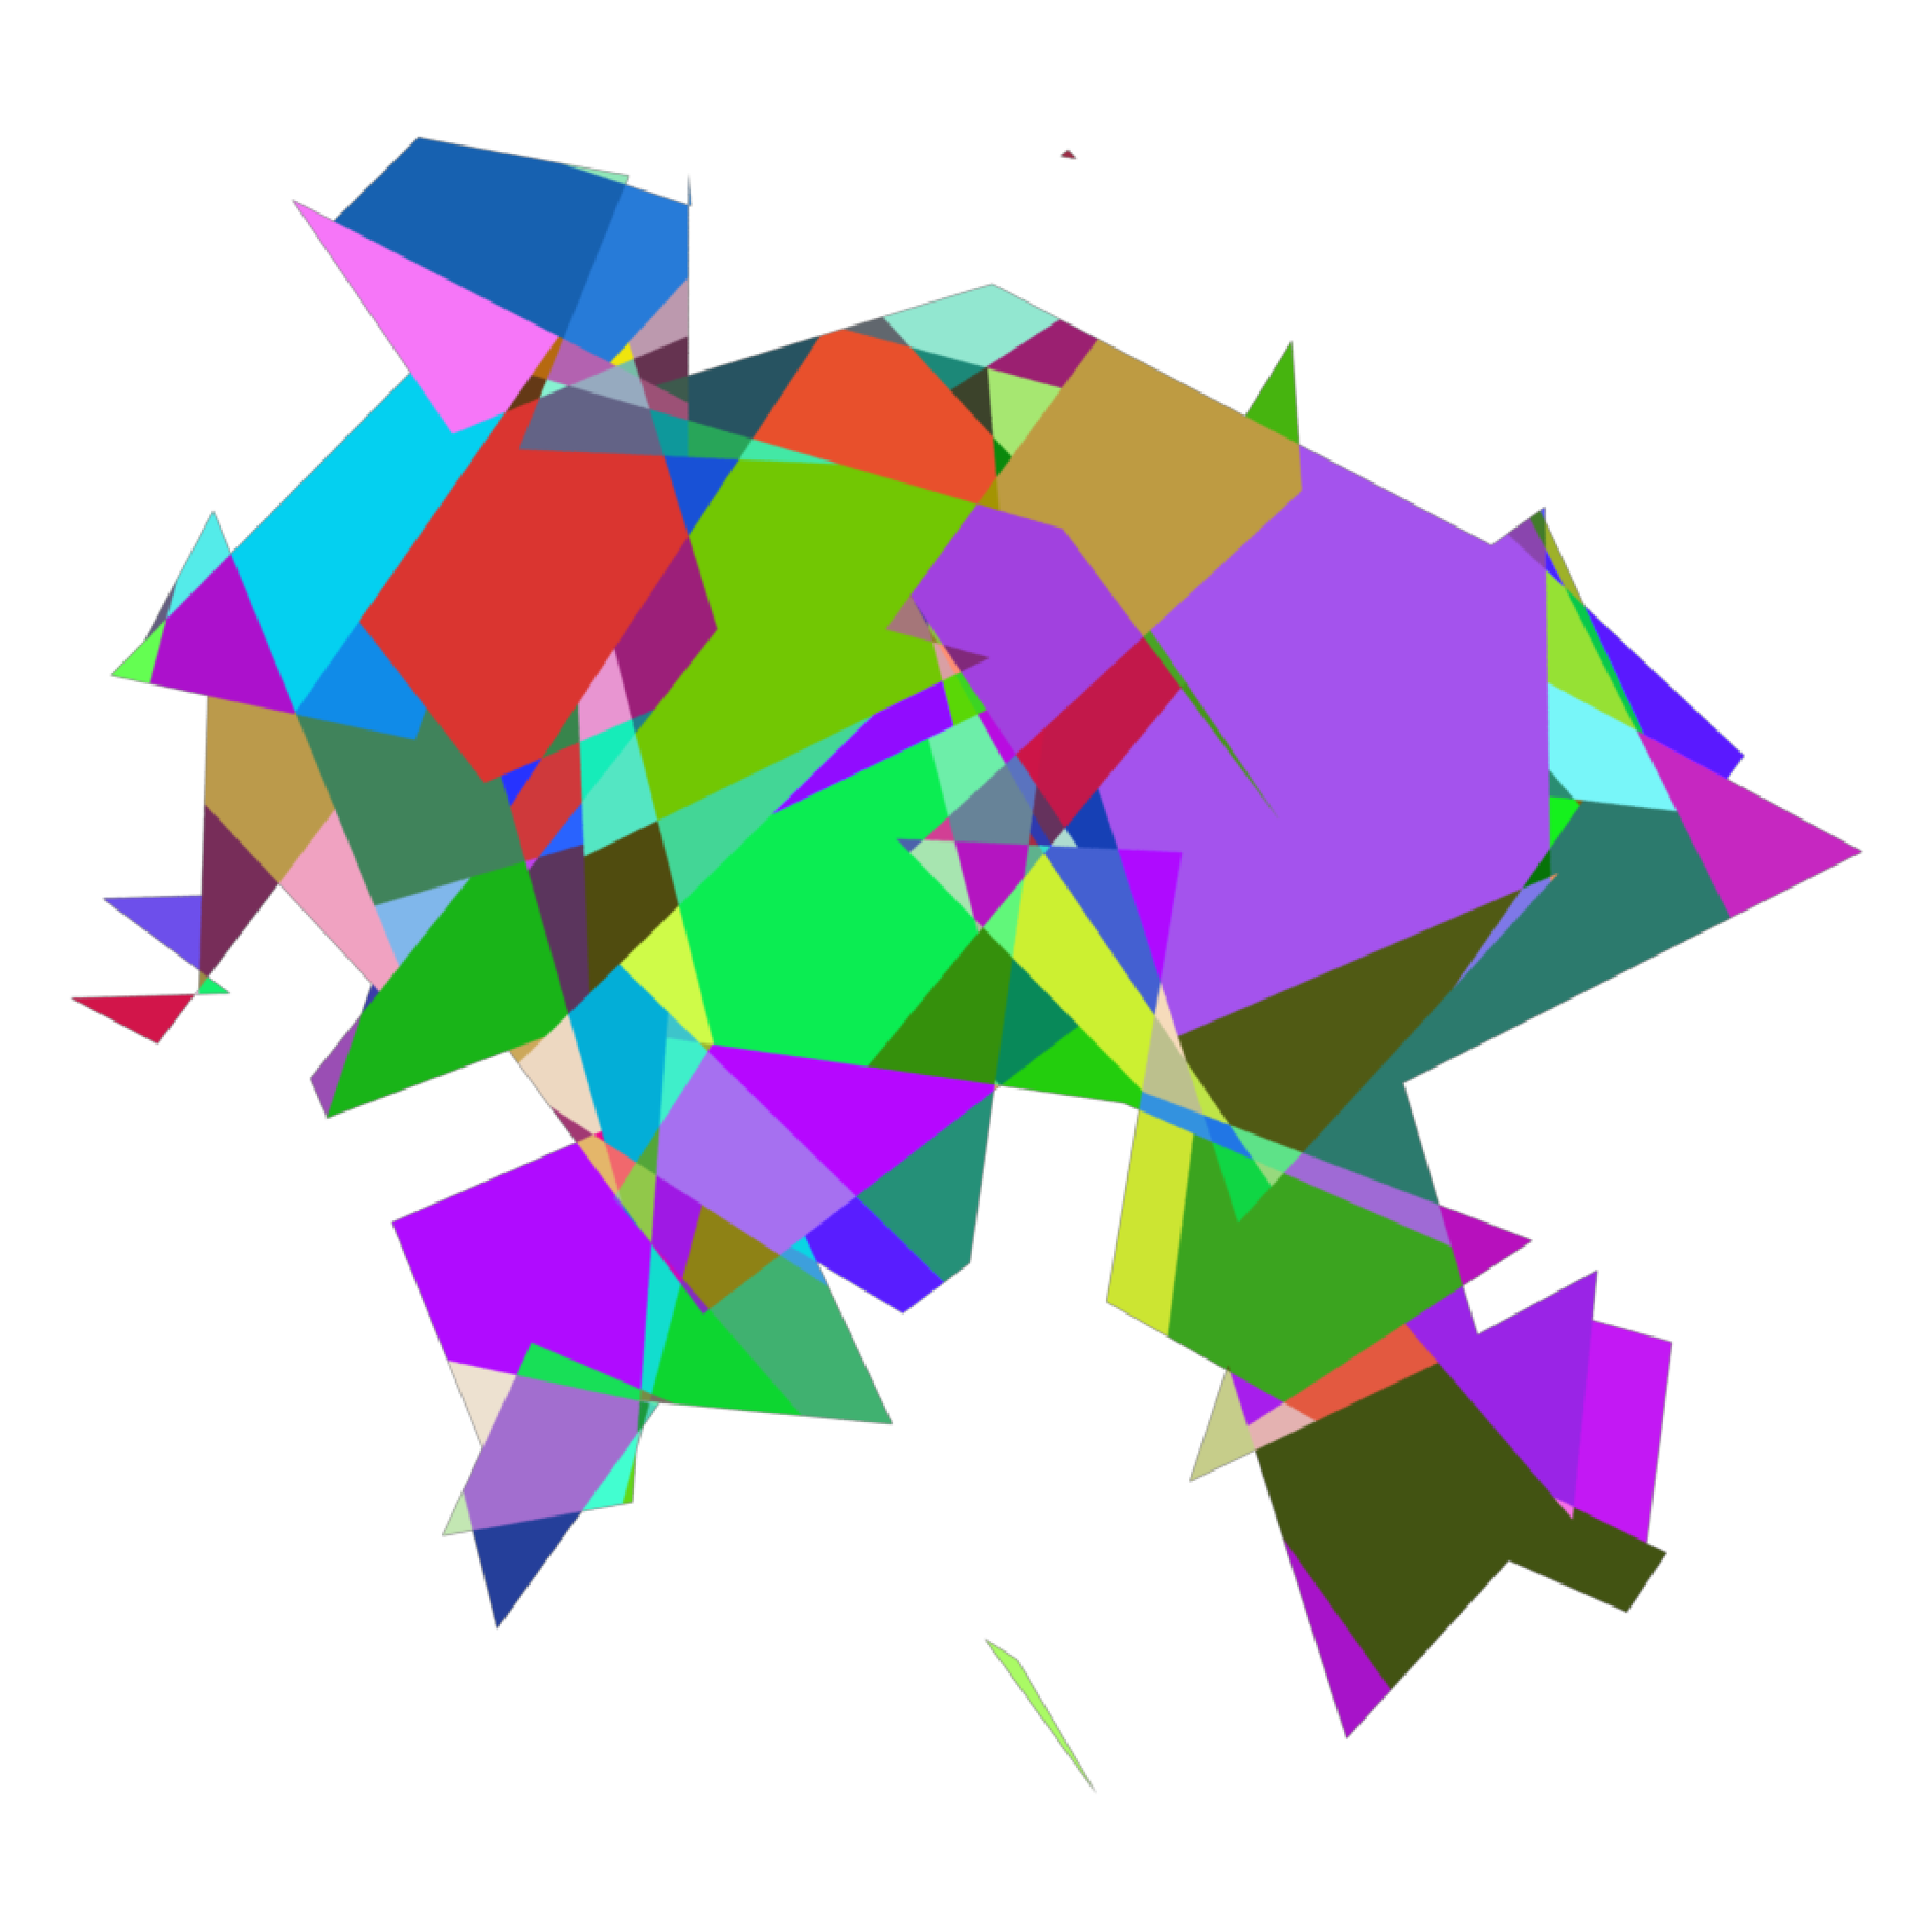
\includegraphics[width=\textwidth]{./img/test-lines-out-compact.pdf}%
    \caption{Output}
\end{figure}

\begin{figure}[p!]
    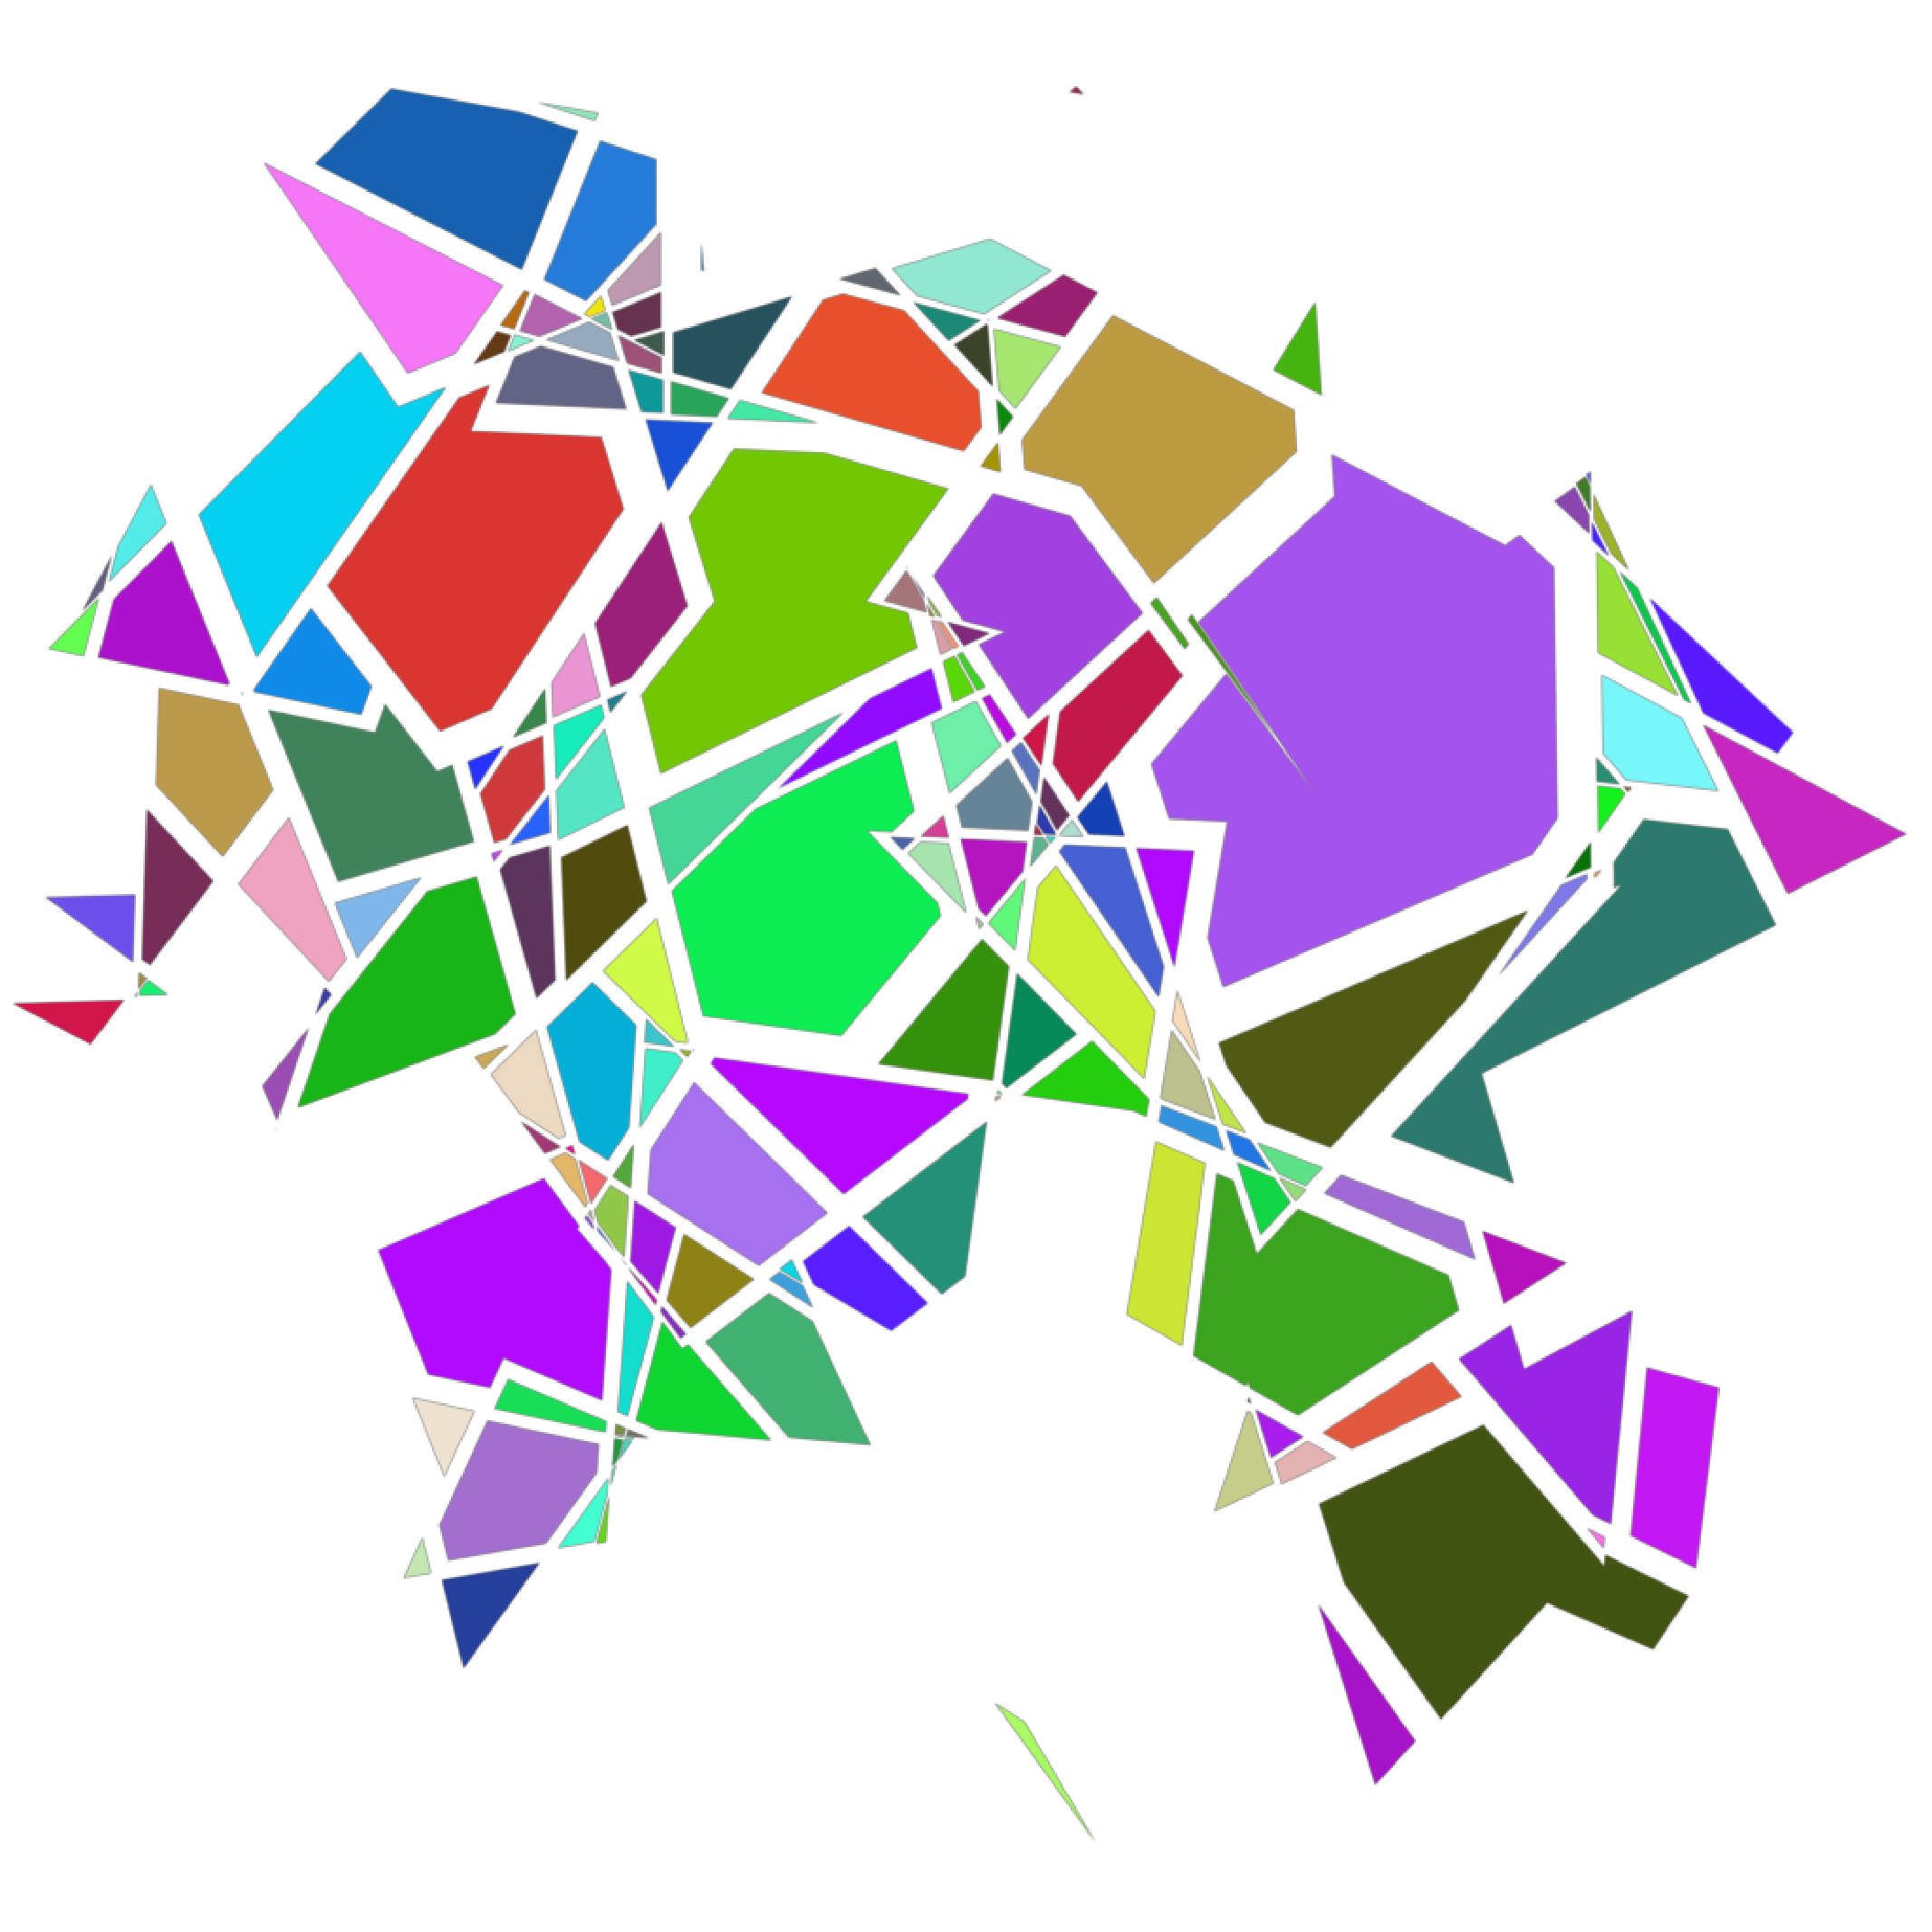
\includegraphics[width=\textwidth]{./img/test-lines-out.pdf}%
    \caption{Output (Exploded)}
\end{figure}

\chapter{Dimension travel}
\label{ch:dimension_travel}

%%%%%%%%%%%%%%%%%%
\section{Overview}

This chapter is dedicated to
the utilities designed to travel
from $\mathbb{E}^3$ to $\mathbb{E}^2$

@O lib/jl/dimension_travel.jl
@{@< Imports and aliases @>
@< Dimension travel functions @>
@}

We will just use the general utilities
in here [ref. \ref{ch:utilities}].

@D Imports and aliases
@{include("./utilities.jl")
@}
%+++++++++++++%
\subsection{Tests}

Some unit tests has been written through development and
they are collected here.

@O test/jl/dimension_travel.jl
@{using Base.Test
include("../../lib/jl/dimension_travel.jl")

@< Tests @>
@}


%%%%%%%%%%%%%%%%%%%%%%%%%%%%%
\section{Submanifold mapping}
\label{sec:submanifold_mapping}

This function, given three points (in $\mathbb{E}^3$), 
returns a $4\times4$ transformation matrix that ``flattens''
the plane defined by the three points onto the $x_3=0$ plane.

@D Dimension travel functions
@{function submanifold_mapping(vs)
    u1 = vs[2,:] - vs[1,:]
    u2 = vs[3,:] - vs[1,:]
    u3 = cross(u1, u2)
    T = eye(4)
    T[4, 1:3] = - vs[1,:]
    M = eye(4)
    M[1:3, 1:3] = [u1 u2 u3]
    return T*M
end
@}
%----------------%
\subsection{Tests}

@D Tests
@{V = rand(3, 3)
m = submanifold_mapping(V)
err = 1e-10 
@@testset "submanifold_mapping test" begin
    @@test any(map((x,y)->-err<x-y<err, m*inv(m), eye(4)))
    @@test any(x->-err<x<err, ([V [1; 1; 1]]*m)[:, 3])
end
@}





%%%%%%%%%%%%%%%%%%%%%%%%%%%%%%%%%%%
\section{Spatial index computation}
\label{sec:spatial_index}

The aim of this function is to compute a \textit{spatial index} that maps
each face to a set of faces which it may collide with.
This is achieved by profuse use of bounding boxes and interval trees. 
We use the interval trees implementation of the \texttt{IntervalTrees.jl} package
\cite{IntervalTrees}.

@D Imports and aliases
@{using IntervalTrees
@}

@D Dimension travel functions
@{function spatial_index(V::Verts, EV::Cells, FE::Cells)
    d = 3
    faces_num = size(FE, 1)
    @< Build the d-IntervalTrees @>
    @< Create the mapping @>
    mapping
end
@}

The basic idea is to ``unfold'' every $d$-dimensional bounding box into $d$ one-dimensional boxes
(which are intervals).
To do so, one interval tree per dimension must be created. 
We build the $d$-trees by firstly building the intervals for each box and then the trees.
In this way we keep in memory the \texttt{boxes1D} array (which contains the intervals) for later use.
Bounding box calculation is performed by the \texttt{bbox} utility [ref. \ref{sec:bboxes}].

@D Build the d-IntervalTrees
@{IntervalsType = IntervalValue{Float64, Int64}
boxes1D = Array{IntervalsType, 2}(0, d)
for fi in 1:faces_num
    vidxs = (abs(FE[fi:fi,:])*abs(EV))[1,:].nzind
    intervals = map((l,u)->IntervalsType(l,u,fi), bbox(V[vidxs, :])...)
    boxes1D = vcat(boxes1D, intervals)
end
trees = mapslices(IntervalTree{Float64, IntervalsType}, sort(boxes1D, 1), 1)
@}

The \textit{spatial index} is returned as an array of 
\texttt{Int64} arrays. The \texttt{intersect\_intervals} 
function returns every cell of which its bounding box collides with 
the $d$-intervals passed as argument. This function 
then is called for the $d$-intervals (stored in the 
\texttt{boxes1D} array) of every cell. Obviously every 
cell collides with itself, so a set difference is 
performed for every cell to exclude itself from the mapping.

@D Create the mapping
@{function intersect_intervals(intervals)
    cells = Array{Int64,1}[]
    for axis in 1:d
        vs = map(i->i.value, intersect(trees[axis], intervals[axis]))
        push!(cells, vs)
    end
    mapreduce(x->x, intersect, cells)
end

mapping = Array{Int64,1}[]
for fi in 1:faces_num
    cell_indexes = setdiff(intersect_intervals(boxes1D[fi, :]), [fi])
    push!(mapping, cell_indexes)
end
@}


%%%%%%%%%%%%%%%%%%%%%%%%%%%%%%%%%%%%%%%%%%%%
\section{Face intersection with $x_3=0$ plane}
\label{sec:face_int}

The intersection of a polygonal face with the $x_3=0$ plane computes
zero, one or more edges. To perform the intersection we find the
intersection point of every edge with the $x_3=0$ plane and then
we connect the points. It is safe to completely ignore edges
parallel to the $x_3=0$ plane.
This is an another procedure where floating-point numbers comparison is
involved and the fixed error rounding is adopted [ref. \ref{sec:floating-point_error}].

@D Dimension travel functions
@{function face_int(V::Verts, EV::Cells, face::Cell)

    vs = buildFV(EV, face)
    retV = Verts(0, 3)
    
    visited_verts = []
    for i in 1:length(vs)
        o = V[vs[i],:]
        j = i < length(vs) ? i+1 : 1
        d = V[vs[j],:] - o

        err = 10e-8
        if !(-err < d[3] < err)

            alpha = -o[3] / d[3]

            if -err <= alpha <= 1+err
                p = o + alpha*d

                if -err < alpha < err || 1-err < alpha < 1+err
                    if !(vin(p, visited_verts))
                        push!(visited_verts, p)
                        retV = [retV; reshape(p, 1, 3)] 
                    end
                else
                    retV = [retV; reshape(p, 1, 3)]
                end
            end
        end

    end

    vnum = size(retV, 1)


    if vnum == 1
        vnum = 0
        retV = Verts(0, 3)
    end
    enum = Int(vnum / 2)
    retEV = spzeros(Int8, enum, vnum)

    for i in 1:enum
        retEV[i, 2*i-1:2*i] = [-1, 1]
    end

    retV, retEV
end
@} 

\chapter{Minimal cycles computation}
\label{ch:minimal_cycles}

\section{Main function}


Computing the minimal cycles means to compute the $d$-boundary matrix
from the $(d-1)$-boundary. The method has been profusely illustrated
by A. Paoluzzi et al. in \textit{Arrangements of cellular complexes}
\cite{Paoluzzi}.
The method is dimension-independent, so works for both $d=2$ and $d=3$;
the only difference between the two cases lays in the \texttt{angles\_fn}
function [ref. \ref{sec:angles_fn}]. To support this multidimensional
behavior, the algorithm has been implemented as an high-order function\footnote{
    \textbf{Notes on variables names:} \texttt{ld} stands for \textit{lower dimension} ($d-1$)
    and \texttt{lld} for \textit{lower lower dimension} ($d-2$). So, \texttt{ld\_cellsnum} is the
    short form of \textit{lower dimension cell number}. For example, if $d=2$, \texttt{ld\_cellsnum} stands for the
    number of $1-$cells, aka the edges.
}:

@O lib/jl/minimal_cycles.jl
@{@< Minimal cycles implementations @>

function minimal_cycles(angles_fn::Function, verbose=false)

    function _minimal_cycles(V::Verts, ld_bounds::Cells)
        @< Function body @>
    end

    return _minimal_cycles
end
@}

In the internal function we store an array of integers called \texttt{count\_marks} 
that increments every time a cells is visited. We do that because to build 
a complete $d$-boundary, we must visit every $(d-1)$-cell exactly twice;
Said so, it appears clear that the algorithm must iterate until a $(d-1)$-cell 
marked with 0 or 1 can be found. Near to \texttt{count\_marks} is stored another
array called \texttt{dir\_marks} that memorizes the direction in which each $(d-1)$-cell
has been visited the last time (this is useful to determine the direction in which the cell
must be visited next). We also print a progression counter for user feedback 
if the \texttt{verbose} flag has been set.

@D Function body
@{lld_cellsnum, ld_cellsnum = size(ld_bounds)
count_marks = zeros(Int8, ld_cellsnum)
dir_marks = zeros(Int8, ld_cellsnum)
d_bounds = spzeros(Int8, ld_cellsnum, 0)

@< minimal\_cycles local variables @>
@< minimal\_cycles utilities @>

while (sigma = get_seed_cell()) > 0

    if verbose
        print(Int(floor(50 * sum(count_marks) / ld_cellsnum)), "%\r")
    end

    @< Compute a cycle @>
end

return d_bounds
@}

The \texttt{get\_seed\_cell} function returns the first $d-1$ cell
marked with zero. If there are no cells marked with zero, the first cell
marked with one will be returned. If every cell is marked with 2 then $-1$
will be returned.

@D minimal\_cycles utilities
@{function get_seed_cell()
    s = -1
    for i in 1:ld_cellsnum
        if count_marks[i] == 0
            return i
        elseif count_marks[i] == 1 && s < 0
            s = i
        end
    end
    return s
end
@}

The bigger part of the algorithm is the computation
of a single cycle. It is mostly equivalent to the
ALGORITHM 1 by A. Paoluzzi et al.
\cite{Paoluzzi}

@D Compute a cycle
@{c_ld = spzeros(Int8, ld_cellsnum)
if count_marks[sigma] == 0
    c_ld[sigma] = 1
else
    c_ld[sigma] = -dir_marks[sigma]
end
c_lld = ld_bounds*c_ld
while c_lld.nzind != []
    corolla = spzeros(Int8, ld_cellsnum)
    for tau in c_lld.nzind
        b_ld = ld_bounds[tau, :]
        pivot = intersect(c_ld.nzind, b_ld.nzind)[1]
        adj = nextprev(tau, pivot, sign(-c_lld[tau]))
        corolla[adj] = c_ld[pivot]
        if b_ld[adj] == b_ld[pivot]
            corolla[adj] *= -1
        end
    end
    c_ld += corolla
    c_lld = ld_bounds*c_ld
end
map(s->count_marks[s] += 1, c_ld.nzind)
map(s->dir_marks[s] = c_ld[s], c_ld.nzind)
d_bounds = [d_bounds c_ld]
@}

This algorithm
revolves around the \textit{next} and \textit{prev} functions. To speed up their
computation, before the cycles iteration starts, we calculate and
store for each ($d-2$)-cell the angles that its incident ($d-1$)-cells
form with it.

@D minimal\_cycles local variables
@{angles = Array{Array{Int64, 1}, 1}(lld_cellsnum)
@}

Here we use the parameter \texttt{angles\_fn::Function}. As explained earlier,
this function is the only difference between the $d=3$ and $d=2$ version of
\texttt{minimal\_cycles}.

@D minimal\_cycles utilities
@{for lld in 1:lld_cellsnum
    as = []
    for ld in ld_bounds[lld, :].nzind
        push!(as, (ld, angles_fn(lld, ld)))
    end
    sort!(as, lt=(a,b)->a[2]<b[2])
    as = map(a->a[1], as)
    angles[lld] = as
end
@}

Once computed the \texttt{angles}, the \texttt{nextprev} function is
easy to implement. The \texttt{norp} parameter is a short form for \textit{next or prev}. 
It determines if the function should choose the first available
($d-1$)-cell rotating clockwise or counterclockwise around the ($d-2$)-cell.

@D minimal\_cycles utilities
@{function nextprev(lld::Int64, ld::Int64, norp)
    as = angles[lld]
    ne = findfirst(as, ld)
    while true
        ne += norp
        if ne > length(as)
            ne = 1
        elseif ne < 1
            ne = length(as)
        end

        if count_marks[as[ne]] < 2
            break
        end
    end
    as[ne]
end
@}



\section{Dimensional wise implementations}
\label{sec:angles_fn}

%%%%%%%%%%%%%%%%%%
\subsection{$d=2$}

When in $d=2$, ($d-2$)-cells are vertices and ($d-1$)-cells are edges.
The \texttt{edge\_angle} function uses the Julia's \texttt{atan2} 
built-in function to calculate the angle of the edge from the vertex point of view.

@D Minimal cycles implementations
@{function minimal_2cycles(V::Verts, EV::Cells)

    function edge_angle(v::Int, e::Int)
        edge = EV[e, :]
        v2 = setdiff(edge.nzind, [v])[1]
        x, y = V[v2, :] - V[v, :]
        return atan2(y, x)
    end

    for i in 1:EV.m
        j = min(EV[i,:].nzind...)
        EV[i, j] = -1
    end
    VE = EV'

    EF = minimal_cycles(edge_angle)(V, VE)

    return EF'
end
@}


%%%%%%%%%%%%%%%%%%
\subsection{$d=3$}
\label{sec:3d_minimal_cycles}

Here we have edges for ($d-2$)-cells and faces for ($d-1$)-cells.

@D Minimal cycles implementations
@{function minimal_3cycles(V::Verts, EV::Cells, FE::Cells)

    @< Face angle function @>

    EF = FE'

    FC = minimal_cycles(face_angle, true)(V, EF)

    return -FC'
end
@}

This time we need to sort faces around an hinge edge.
To compute the angle of a face, we transform it
in a way that the hinge lays on the $x_1$ positive
axis\footnote{The method to compute an univocal reference frame 
from a single vector comes from \textit{Physically Based Rendering} by
Pharr and Humphreys \cite{Pharr:2010:PBR:1854996}}. In this way, 
we can compute the angle of a face
by using a classic \texttt{atan2} call. 

Due to the fact that faces can be non-convex, 
we triangulate them to be sure to compute their 
angle correctly; in the case of a non-convex face, 
it can happen that is picked erroneously the opposite
angle of the right one. The triangulation is performed
only when the face of index \texttt{f} is visited for the first time.


@D Face angle function
@{triangulated_faces = Array{Any, 1}(FE.m)

function face_angle(e::Int, f::Int)
    if !isassigned(triangulated_faces, f)
        @< Triangulate face @>
    end

    edge_vs = EV[e, :].nzind

    t = findfirst(x->edge_vs[1] in x && edge_vs[2] in x, triangulated_faces[f])
    
    v1 = normalize(V[edge_vs[2], :] - V[edge_vs[1], :])
    if abs(v1[1]) > abs(v1[2])
        invlen = 1. / sqrt(v1[1]*v1[1] + v1[3]*v1[3])
        v2 = [-v1[3]*invlen, 0, v1[1]*invlen]
    else
        invlen = 1. / sqrt(v1[2]*v1[2] + v1[3]*v1[3])
        v2 = [0, -v1[3]*invlen, v1[2]*invlen]
    end
    v3 = cross(v1, v2)

    M = reshape([v1; v2; v3], 3, 3)

    triangle = triangulated_faces[f][t]
    third_v = setdiff(triangle, edge_vs)[1]
    vs = V[[edge_vs..., third_v], :]*M

    v = vs[3, :] - vs[1, :]
    angle = atan2(v[2], v[3]) 

    return angle
end
@}

To perform triangulation we use the
Julia porting by F. Furiani of Triangle, 
a well known C library for constrained 
Delaunay triangulations \cite{Triangle.jl}\cite{Triangle}.
Due to the fact that Delaunay triangulation works only
in $\mathbb{E}^2$, we need to transform the face to triangulate
on the $x_3=0$ plane. To compute a reference frame on the
face plane, we use the classic method of doing two differences 
of three non-colinear vertices of the face
and then cross multiply the vectors resulting from the differences
two to get a third one.
To make sure that the three chosen vertices are not colinear, we
check if the cross of the two difference vectors has non-zero length
and we choose new set of vertices until this condition is satisfied%
\footnote{We check the length of the cross product against a fixed
error [ref. \ref{sec:floating-point_error}].}.

@D LAR imports
@{using TRIANGLE
@}

@D Triangulate face
@{vs_idxs = Array{Int64, 1}()
edges_idxs = FE[f, :].nzind
edge_num = length(edges_idxs)
edges = zeros(Int64, edge_num, 2)

for (i, ee) in enumerate(edges_idxs)
    edge = EV[ee, :].nzind
    edges[i, :] = edge
    vs_idxs = union(vs_idxs, edge)
end

vs = V[vs_idxs, :]

v1 = normalize(vs[2, :] - vs[1, :])
v3 = [0 0 0]
err = 1e-8
i = 3
while -err < norm(v3) < err
    v2 = normalize(vs[i, :] - vs[1, :])
    v3 = cross(v1, v2)
    i = i + 1
end

M = reshape([v1; v2; v3], 3, 3)

vs = vs*M

triangulated_faces[f] = TRIANGLE.constrained_triangulation(
    vs, vs_idxs, edges, fill(true, edge_num))
@}
\chapter{Utilities}
\label{ch:utilities}

%%%%%%%%%%%%%%%%%%
\section{Overview}

The functionalities shared between all the components of LAR
are defined in here.

@O lib/jl/utilities.jl
@{@< LAR types @>
@< Utilities @>
@}

\subsection{Tests}
As usual every function has some unit tests.

@O test/jl/utilities.jl
@{using Base.Test
include("../../lib/jl/utilities.jl")

@< Utilities tests @>
@}

%%%%%%%%%%%%%%%
\section{Standard types}

We define at the top of our module the standard types
that will be used throughout LAR. As already explained
in the introduction [ref. \ref{sec:LAR}], LAR needs
only one bi-dimensional array to store geometry and 
one or more sparse matrices for topology.
Julia has already implemented CSC sparse matrices in
its standard library so we are going to use them.

@D LAR types
@{const Verts = Array{Float64, 2}
const Cells = SparseMatrixCSC{Int8, Int}
const Cell = SparseVector{Int8, Int}
@}

We used the general name \texttt{Cells}, but
we are going to use this type also for boundaries.

\subsection{Floating point error}
\label{sec:floating-point_error}

We stored geometry using 64-bit IEEE floats.
As it is known, floating point arithmetic is not
precise and introduces numerical errors.
Usually this is not an issue\footnote{The \textit{machine epsilon},
which is the upper bound on the relative error in floating-point 
arithmetic, for double precision IEEE floating-point numbers is 
$2^53 \approx 1.11 \times 10^{-16}$.}, but when precision is
a goal, floating point error must be handled very carefully.
During the development we encountered several numerical problems
and we tried various approaches (like normalizing the geometry
inside the $[0, 1]$ interval for each dimension in order to maximize
the significand of the floating-point numbers) but most of them turned 
out to be unstable. So we choose the less orthodox path we could
possibly take: we set a fixed error and we performed every floating point
comparison using this error. Examples of this ``tweak'' are to be found in
\ref{sec:intersect_edges}, \ref{sec:face_int}, \ref{sec:3d_minimal_cycles} and 
\ref{sec:vertex_equality}.


%%%%%%%%%%%%%%%%%%%%%%%%
\section{Bounding boxes}
\label{sec:bboxes}

Bounding boxes are essential in many steps of many
algorithms in LAR. Here we present a method for building
and performing containment tests on n-dimensional 
axis aligned bounding boxes.

@D Utilities
@{function bbox(vertices::Verts)
    minimum = mapslices(x->min(x...), vertices, 1)
    maximum = mapslices(x->max(x...), vertices, 1)
    minimum, maximum
end

function bbox_contains(container, contained)
    b1_min, b1_max = container
    b2_min, b2_max = contained
    all(map((i,j,k,l)->i<=j<=k<=l, b1_min, b2_min, b2_max, b1_max))
end
@}

\subsection{Tests}
\begin{figure}[h]
    \centering
    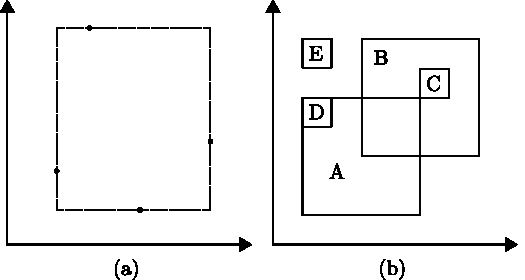
\includegraphics{./img/ch5-bboxes.pdf}
    \caption{(a) is a visualization of the test for bboxes building, (b) for bbox containment.}
\end{figure}
@D Utilities tests
@{@@testset "Bounding boxes building test" begin
    V = [.56 .28; .84 .57; .35  1.0; .22  .43]
    @@test bbox(V) == ([.22 .28], [.84 1.0])
end

@@testset "Bounding boxes containment test" begin
    bboxA = ([0. 0.], [1. 1.])
    bboxB = ([.5 .5], [1.5 1.5])
    bboxC = ([1. 1.], [1.25 1.25])
    bboxD = ([0 .75], [.25 1])
    bboxE = ([0 1.25], [.25 1.5])

    @@test bbox_contains(bboxA, bboxD)
    @@test bbox_contains(bboxB, bboxC)
    @@test !bbox_contains(bboxA, bboxB)
    @@test !bbox_contains(bboxA, bboxE)
end
@}

%%%%%%%%%%%%%%%%%%%%%%%%%%%%%%%
\section{Face area calculation}
\label{sec:face_area}

\begin{figure}[h]
    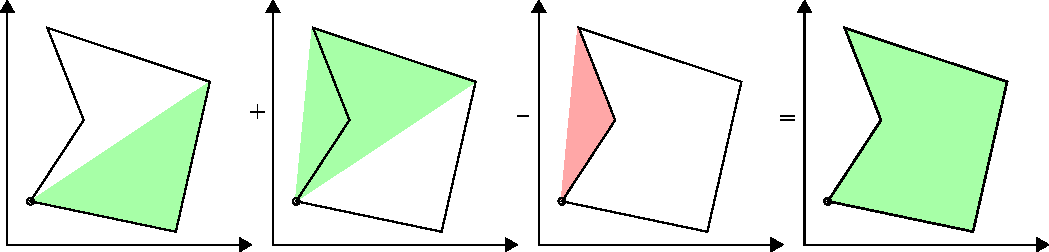
\includegraphics[width=\textwidth]{./img/ch5-area.pdf}
    \caption{A visual representation of the face area calculation algorithm. The area
    of the face is the sum of the areas of each triangle which can be build using the 
    pivot vertex and the other vertices of the face}
\end{figure}
\noindent
To compute the area of a generic (convex or concave) face,
we pick a pivot vertex of the face and then we iterate over
every edge of the face calculating the area of the triangle
made by the pivot vertex and the ordered extremes of the current edge.
The area of the full face is the sum of the areas of the single triangles.
This works because of the single triangles we compute the signed area with
this formula:
\begin{gather*}
    A = \frac{1}{2}
    \begin{vmatrix}
        p_{1x} & p_{1y} & 1 \\
        p_{2x} & p_{2y} & 1 \\
        p_{3x} & p_{3y} & 1
    \end{vmatrix}
\end{gather*}
Where $p_1$, $p_2$ and $p_3$ are the vertices of the triangle ($p_1$ is the pivot vertex). 
Please notice that the result of this formula will be negative only if these vertices 
are arranged in clockwise order.

@D Utilities
@{function face_area(V::Verts, EV::Cells, face::Cell)
    function triangle_area(triangle_points::Verts)
        ret = ones(3,3)
        ret[:, 1:2] = triangle_points
        return .5*det(ret)
    end

    area = 0

    fv = buildFV(EV, face)

    verts_num = length(fv)
    v1 = fv[1]

    for i in 2:(verts_num-1)

        v2 = fv[i]
        v3 = fv[i+1]

        area += triangle_area(V[[v1, v2, v3], :])
    end

    return area
end
@}

\subsection{Tests}
\begin{figure}[h]
    \centering
    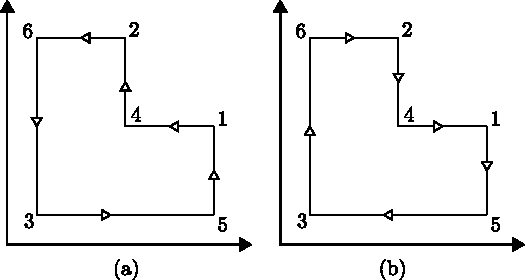
\includegraphics{./img/ch5-area_test.pdf}
\end{figure}
\noindent The two faces drawn above they must have complimentary area.
@D Utilities tests
@{@@testset "Face area calculation test" begin
    V = Float64[2 1; 1 2; 0 0; 1 1; 2 0; 0 2]
    EV = spzeros(Int8, 6, 6)
    EV[1, [1, 4]] = [-1, 1]; EV[2, [2, 4]] = [-1, 1]
    EV[3, [2, 6]] = [-1, 1]; EV[4, [3, 6]] = [-1, 1]
    EV[5, [3, 5]] = [-1, 1]; EV[6, [1, 5]] = [-1, 1]
    FE = spzeros(Int8, 2, 6)
    FE[1, :] = [ 1 -1  1 -1  1 -1]
    FE[2, :] = [-1  1 -1  1 -1  1]

    @@test face_area(V, EV, FE[1,:]) == -face_area(V, EV, FE[2,:])
end
@}

%%%%%%%%%%%%%%%%%%%%%%%%
\section{Skeletal merge}
\label{sec:skel_merge}

The first step of the arrangement algorithm is ever
the skeletal merge [ref. \ref{sec:spatial_arrangement_overview}].

@D Utilities
@{function skel_merge(V1::Verts, EV1::Cells, V2::Verts, EV2::Cells)
    V = [V1; V2]
    EV = spzeros(Int8, EV1.m + EV2.m, EV1.n + EV2.n)
    EV[1:EV1.m, 1:EV1.n] = EV1
    EV[EV1.m+1:end, EV1.n+1:end] = EV2
    V, EV
end

function skel_merge(V1::Verts, EV1::Cells, FE1::Cells, V2::Verts, EV2::Cells, FE2::Cells)
    FE = spzeros(Int8, FE1.m + FE2.m, FE1.n + FE2.n)
    FE[1:FE1.m, 1:FE1.n] = FE1
    FE[FE1.m+1:end, FE1.n+1:end] = FE2
    V, EV = skel_merge(V1, EV1, V2, EV2)
    V, EV, FE
end
@}

%%%%%%%%%%%%%%%%%%%%%%%
\section{Edge deletion}
\label{sec:delete_edges}

Deleting edges ia a common operation in planar arrangement. When
edges are deleted, some vertices can remain unconnected; these must be deleted too.

@D Utilities
@{function delete_edges(todel, V::Verts, EV::Cells)
    tokeep = setdiff(collect(1:EV.m), todel)
    EV = EV[tokeep, :]
    
    vertinds = 1:EV.n
    todel = Array{Int64, 1}()
    for i in vertinds
        if length(EV[:, i].nzind) == 0
            push!(todel, i)
        end
    end

    tokeep = setdiff(vertinds, todel)
    EV = EV[:, tokeep]
    V = V[tokeep, :]

    return V, EV
end
@}


%%%%%%%%%%%%%%%%%%%%%%%
\section{FV building}

Sometimes is useful to represent a face like a sequence of vertices.

@D Utilities
@{function buildFV(EV::Cells, face::Cell)
    startv = -1
    nextv = 0
    edge = 0

    vs = Array{Int64, 1}()

    while startv != nextv
        if startv < 0
            edge = face.nzind[1]
            startv = EV[edge,:].nzind[face[edge] < 0 ? 2 : 1]
            push!(vs, startv)
        else
            edge = setdiff(intersect(face.nzind, EV[:, nextv].nzind), edge)[1]
        end
        nextv = EV[edge,:].nzind[face[edge] < 0 ? 1 : 2]
        push!(vs, nextv)

    end

    return vs[1:end-1]
end
@}


%%%%%%%%%%%%%%%%%%%%%%
\section{Boundaries building}

@D Utilities
@{function buildFE(FV, edges)
    faces = []

    for face in FV
        f = []
        for (i,v) in enumerate(face)
            edge = [v, face[i==length(face)?1:i+1]]
            ord_edge = sort(edge)

            edge_idx = findfirst(e->e==ord_edge, edges)

            push!(f, (edge_idx, sign(edge[2]-edge[1])))
        end
        
        push!(faces, f)
    end

    FE = spzeros(Int8, length(faces), length(edges))

    for (i,f) in enumerate(faces)
        for e in f
            FE[i, e[1]] = e[2]
        end
    end

    return FE
end

function buildEV(edges)
    maxv = max(map(x->max(x...), edges)...)
    EV = spzeros(Int8, length(edges), maxv)

    for (i,e) in enumerate(edges)
        e = sort(collect(e))
        EV[i, e] = [-1, 1]
    end

    return EV
end


function buildFV(EV::Cells, face)
    startv = face[1]
    nextv = startv

    vs = []
    visited_edges = []

    while true
        curv = nextv
        push!(vs, curv)

        edge = 0
        for edge in EV[:, curv].nzind
            nextv = setdiff(EV[edge, :].nzind, curv)[1]
            if nextv in face && (nextv == startv || !(nextv in vs)) && !(edge in visited_edges)
                break
            end
        end

        push!(visited_edges, edge)

        if nextv == startv
            break
        end
    end

    return vs
end


function build_bounds(edges, faces)
    EV = buildEV(edges)
    FV = map(x->buildFV(EV,x), faces)
    FE = buildFE(FV, edges)

    return EV, FE
end
@}


%%%%%%%%%%%%%%%%%%%%%
\section{Vertex equality utilities}
\label{sec:vertex_equality}

Vertex comparison must be performed using 
floating-point fixed error 
[ref. \ref{sec:floating-point_error}].

@D Utilities
@{function vin(vertex, vertices_set)
    for v in vertices_set
        if vequals(vertex, v)
            return true
        end
    end
    return false
end

function vequals(v1, v2)
    err = 10e-8
    return length(v1) == length(v2) && all(map((x1, x2)->-err < x1-x2 < err, v1, v2))
end
@}

%%%%%%%%%%%%%%%%%%%%%%%%%%%
\section{Full triangulation}


@D Utilities
@{function triangulate(V::Verts, EV::Cells, FE::Cells)

    triangulated_faces = Array{Any, 1}(FE.m)

    for f in 1:FE.m
        if f % 10 == 0
            print(".")
        end
        
        edges_idxs = FE[f, :].nzind
        edge_num = length(edges_idxs)
        edges = zeros(Int64, edge_num, 2)

        
        fv = buildFV(EV, FE[f, :])

        vs = V[fv, :]

        v1 = normalize(vs[2, :] - vs[1, :])
        v2 = [0 0 0]
        v3 = [0 0 0]
        err = 1e-8
        i = 3
        while -err < norm(v3) < err
            v2 = normalize(vs[i, :] - vs[1, :])
            v3 = cross(v1, v2)
            i = i + 1
        end
        M = reshape([v1; v2; v3], 3, 3)

        vs = (vs*M)[:, 1:2]
        tV = (V*M)[:, 1:2]

        area = face_area(tV, EV, FE[f, :])
        if area > 0 
            fv = fv[end:-1:1]
        end
        
        for i in 1:length(fv)
            edges[i, 1] = fv[i]
            edges[i, 2] = i == length(fv) ? fv[1] : fv[i+1]
        end
        
        triangulated_faces[f] = TRIANGLE.constrained_triangulation(vs, fv, edges, fill(true, edge_num))
    end

    return triangulated_faces
end
@}


%%%%%%%%%%%%%%%%%%%%%
\section{OBJ I/O}

OBj is a common format for 3D models exchange. 
Here an exporter of LAR model to OBJ. It returns a string.

@D Utilities
@{function lar2obj(V::Verts, EV::Cells, FE::Cells, CF::Cells)
    obj = ""
    for v in 1:size(V, 1)
        obj = string(obj, "v ", round(V[v, 1], 6), " ", round(V[v, 2], 6), " ", round(V[v, 3], 6), "\n")
    end

    print("Triangulating")
    triangulated_faces = triangulate(V, EV, FE)
    println("DONE")

    for c in 1:CF.m
        obj = string(obj, "\ng cell", c, "\n")
        for f in CF[c, :].nzind
            triangles = triangulated_faces[f]
            for tri in triangles
                t = CF[c, f] > 0 ? tri : tri[end:-1:1]
                obj = string(obj, "f ", t[1], " ", t[2], " ", t[3], "\n")
            end
        end
    end

    return obj
end
@}

And here an importer. It wants a path to the obj file
expressed as a string. It returns the classic tuple \texttt{V, EV, FE}.

@D Utilities
@{function obj2lar(path)
    fd = open(path, "r")
    vs = Array{Float64, 2}(0, 3)
    edges = Array{Array{Int, 1}, 1}()
    faces = Array{Array{Int, 1}, 1}()

    while (line = readline(fd)) != ""
        elems = split(line)
        if length(elems) > 0
            if elems[1] == "v"

                x = parse(Float64, elems[2])
                y = parse(Float64, elems[3])
                z = parse(Float64, elems[4])
                vs = [vs; x y z]

            elseif elems[1] == "f"
                v1 = parse(Int, elems[2])
                v2 = parse(Int, elems[3])
                v3 = parse(Int, elems[4])

                e1 = sort([v1, v2])
                e2 = sort([v2, v3])
                e3 = sort([v1, v3])

                if !(e1 in edges)
                    push!(edges, e1)
                end
                if !(e2 in edges)
                    push!(edges, e2)
                end
                if !(e3 in edges)
                    push!(edges, e3)
                end

                push!(faces, sort([v1, v2, v3]))
            end
        end
    end

    close(fd)
    vs, build_bounds(edges, faces)...
end  
@}


%%%%%%%%%%%%%%%%%%%%%%
\section{Point in face area}
\label{sec:point_in_face}

Point in face inclusion is performed using the algorithm
presented by A. Paoluzzi in 1986 \cite{Paoluzzi-ART1986}.
It is based on the ray shooting and it analyzes more than
thirty possible ray-edge intersection cases.

@D Utilities
@{function point_in_face(origin, V::Verts, ev::Cells)

    function pointInPolygonClassification(V,EV)

        function crossingTest(new, old, status, count)
        if status == 0
            status = new
            return status, (count + 0.5)
        else
            if status == old
                return 0, (count + 0.5)
            else
                return 0, (count - 0.5)
            end
        end
        end

        function setTile(box)
        tiles = [[9,1,5],[8,0,4],[10,2,6]]
        b1,b2,b3,b4 = box
        function tileCode(point)
            x,y = point
            code = 0
            if y>b1 code=code|1 end
            if y<b2 code=code|2 end
            if x>b3 code=code|4 end
            if x<b4 code=code|8 end
            return code
        end
        return tileCode
        end

        function pointInPolygonClassification0(pnt)
            x,y = pnt
            xmin,xmax,ymin,ymax = x,x,y,y
            tilecode = setTile([ymax,ymin,xmax,xmin])
            count,status = 0,0

            for k in 1:EV.m
                edge = EV[k,:]
                p1, p2 = V[edge.nzind[1], :], V[edge.nzind[2], :]
                (x1,y1),(x2,y2) = p1,p2
                c1,c2 = tilecode(p1),tilecode(p2)
                c_edge, c_un, c_int = xor(c1, c2), c1|c2, c1&c2
                
                if (c_edge == 0) & (c_un == 0) return "p_on" 
                elseif (c_edge == 12) & (c_un == c_edge) return "p_on"
                elseif c_edge == 3
                    if c_int == 0 return "p_on"
                    elseif c_int == 4 count += 1 end
                elseif c_edge == 15
                    x_int = ((y-y2)*(x1-x2)/(y1-y2))+x2 
                    if x_int > x count += 1
                    elseif x_int == x return "p_on" end
                elseif (c_edge == 13) & ((c1==4) | (c2==4))
                        status, count = crossingTest(1,2,status,count)
                elseif (c_edge == 14) & ((c1==4) | (c2==4))
                        status, count = crossingTest(2,1,status,count)
                elseif c_edge == 7 count += 1
                elseif c_edge == 11 count = count
                elseif c_edge == 1
                    if c_int == 0 return "p_on"
                    elseif c_int == 4 
                        status, count = crossingTest(1,2,status,count) 
                    end
                elseif c_edge == 2
                    if c_int == 0 return "p_on"
                    elseif c_int == 4 
                        status, count = crossingTest(2,1,status,count) 
                    end
                elseif (c_edge == 4) & (c_un == c_edge) return "p_on"
                elseif (c_edge == 8) & (c_un == c_edge) return "p_on"
                elseif c_edge == 5
                    if (c1==0) | (c2==0) return "p_on"
                    else 
                        status, count = crossingTest(1,2,status,count) 
                    end
                elseif c_edge == 6
                    if (c1==0) | (c2==0) return "p_on"
                    else 
                        status, count = crossingTest(2,1,status,count) 
                    end
                elseif (c_edge == 9) & ((c1==0) | (c2==0)) return "p_on"
                elseif (c_edge == 10) & ((c1==0) | (c2==0)) return "p_on"
                end
            end
            
            if (round(count)%2)==1 
                return "p_in"
            else 
                return "p_out"
            end
        end
        return pointInPolygonClassification0
    end
    
    return pointInPolygonClassification(V, ev)(origin) == "p_in"
end
@}

\backmatter


\bibliography{book}{}
\bibliographystyle{plain}
\end{document}